\chapter{调度动态可定制沙箱设计与实现}\label{chap:control_zone}

为解决单一调度机制与多样混部场景矛盾的问题,本章设计实现了Contorl Zone,一种面向混部场景的调度动态可定制沙箱。Control Zone基于KVM虚拟机实现,并支持以容器的形式协同部署Control Tower任务调度策略与混部应用。一方面能够针对混部场景量身定制调度策略,另一方面借助BPF技术的动态性实现运行时可变的调度策略。同时,Control Zone还支持丰富的软硬件手段来对资源进行隔离,以提供精细的Control Zone资源分配。

\section{调度动态可定制沙箱Control Zone设计}

% 概述 -> 设计思路

% 介绍 Control Zone 的概念
% - 面对什么场景
% - 存在哪些问题
%   - 复杂的硬件环境
%   - 复杂的软件环境
% - 针对每个问题的解决方式
% - 设计目标

服务器资源丰富,支持大量应用同时运行,这些应用构成了多样的混部场景。然而Linux提供的调度策略有限,难以覆盖每个混部场景。同时,由于应用共享同一个内核,因此调整调度策略时容易对其他应用造成影响。此外,围绕混部场景的任务调度研究通常也只关注有限的混部场景,提供的调度机制或算法在扩展性及灵活性上存在缺陷。而为解决单一调度机制与多样混部场景矛盾,实现单个机器上多种调度机制共存,本文提出了Control Zone,一种基于KVM的面向混部场景的调度动态可定制沙箱。

航空领域中Control Zone指受控空域的一部分,通常在机场的周围负责保护进出的空中交通。Control Zone中由Control Tower进行客机起降的调度,同时Black Box提供了客机飞行数据的监测。本文借用航空领域的上述概念设计Control Zone,具体架构如图~\ref{fig:cz_arch}所示,包含三个主要部分:Control Zone虚拟机、Control Zone管理器、Black Box观测系统。

\begin{figure}[!htbp]
    \centering
    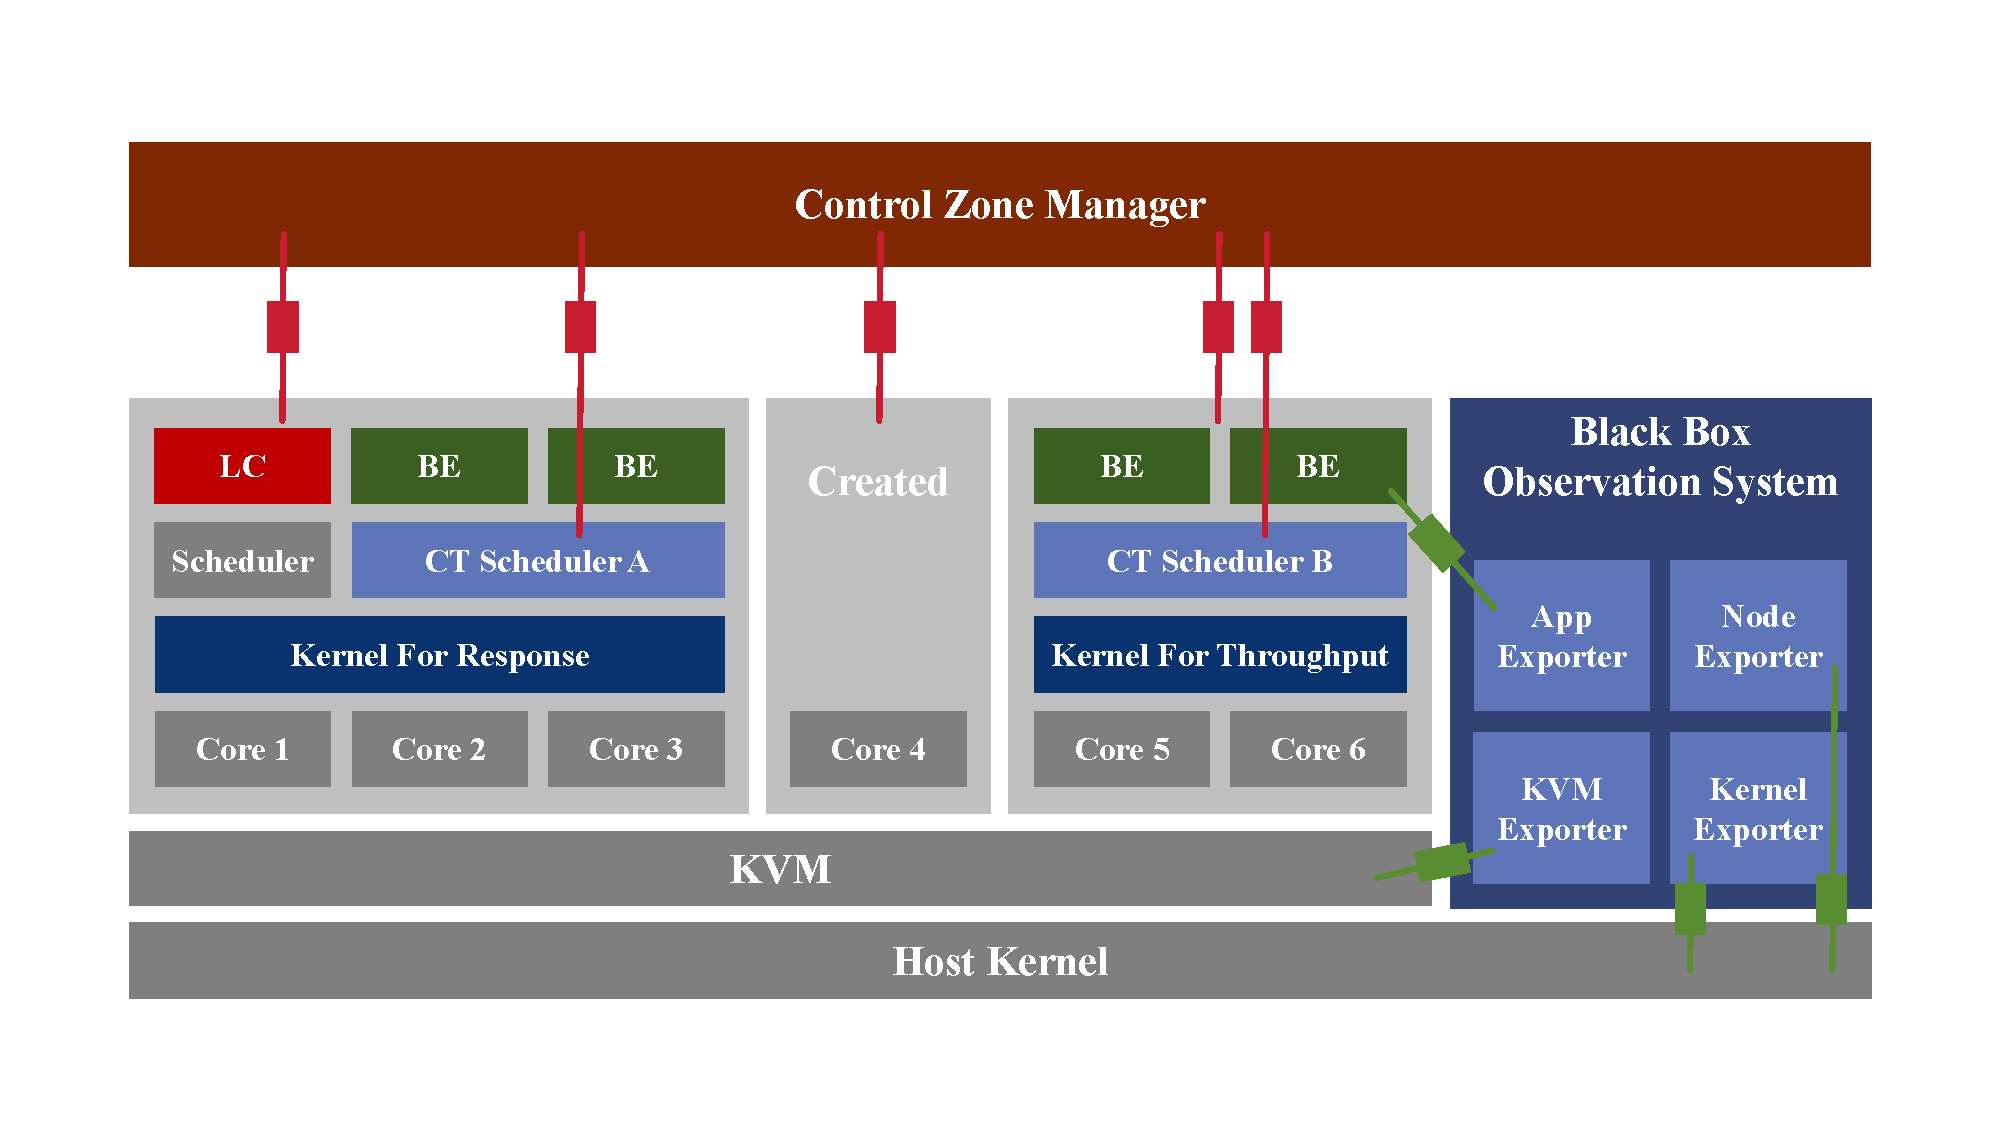
\includegraphics[width=0.9\textwidth]{cz_arch}
    \bicaption{\quad Control Zone基本架构}{\quad Architecture of Control Zone}
    \label{fig:cz_arch}
\end{figure}

\begin{itemize}

    \item \textbf{Control Zone虚拟机}:基于KVM虚拟机实现,同时支持部署容器化的混部应用,并进行混部应用的生命周期管理。Control Zone虚拟机还支持Control Tower调度框架,允许针对混部场景量身定制调度策略,并借助BPF技术的插件化能力实现内核调度策略的运行时动态变化。此外,Control Tower调度策略被封装为容器镜像,并与混部应用一同进行管理。

    \item \textbf{Control Zone管理器}:负责Control Zone虚拟机的生命周期管理,包括Control Zone虚拟机的创建、启动、暂停、销毁等。Control Zone管理器还支持丰富的资源隔离措施,便于控制分配给Control Zone虚拟机的资源。

    \item \textbf{Black Box观测系统}:能够从Host、Hypervisor、App三个层次围绕虚拟机采集丰富的指标,并提供实时的监测与离线的数据分析功能。Black Box观测系统提供了一种持续对Control Zone进行性能分析的方式,一方面有助于了解混部应用的性能,另一方面可协助对调度策略的持续迭代。

\end{itemize}

针对混部场景下软硬件对于任务调度机制的需求。首先,Control Zone可利用虚拟化来屏蔽底层硬件差异,或定制Control Tower调度策略来满足不同硬件的对调度需求。其次,Control Zone允许选择合适的内核调度配置,来满足高优先任务在响应度或吞吐量上的需求。同时,Control Zone允许针对混部场景的量身定制Control Tower调度策略,来满足不同的调度目标。最后,考虑到混部应用负载的以及硬件环境的动态特性,Control Zone提供了一种在运行时切换不同调度策略的方式,而无需中断虚拟机的运行。

\section{调度动态可定制沙箱Control Zone实现}

\subsection{Control Zone轻量级虚拟机}

% 隔离性实现
% 内核裁切
% hypervisor选择
% 系统功能要求
% 镜像共享

Control Zone中使用KVM虚拟机主要出于隔离性与安全性两方面的考虑。在隔离性上,使用KVM虚拟机能够实现较强的隔离效果,同时利用Hypervisor对模拟设备控制能力可提供更丰富的资源隔离手段。在安全性上,修改调度子系统是较危险的行为,并可能影响到系统中的所有任务。使用虚拟机能够将风险限制在单个虚拟机内,此外,借助虚拟机的隔离性使得在一个物理机上同时运行多种不同调度机制成为可能。

引入虚拟机会导致额外的虚拟化开销,主要来自于虚拟机监视器与来宾操作系统。虚拟机监视器要在启动虚拟机之前完成一系列的准备工作,包括各种模拟设备的创建与初始化,这些过程都会增加虚拟机的启动时间。此外,在虚拟机运行过程中,KVM模块无法处理的陷出事件需要转交虚拟机监视器处理,如对部分特殊设备的模拟,这一过程会降低虚拟机的运行速度。来宾操作系统是应用运行的基本环境,虚拟机中,操作系统启动以及运行时消耗的资源都是额外开销。此外对于容器化应用而言,容器运行时所消耗的资源同样也是一种额外开销。

虚拟化开销显著影响了沙箱的性能,增加了保障混部应用QoS的困难。而Control Zone使用KVM虚拟机仅为提供较强的隔离环境,且综合上述分析发现绝大部分开销是不必要的。因此为减少虚拟化开销,本文设计实现了Control Zone轻量级虚拟机,从虚拟机监视器、来宾操作系统和容器运行时三个方面优化沙箱开销:

\begin{itemize}

    \item \textbf{轻量化的虚拟机监视器}:Control Zone在CloudHypervisor的基础上构建轻量级虚拟机监视器。CloudHypervisor与Firecracker类似,都是基于Rust-VMM套件构建的轻量级虚拟机监视器。相比于Firecracker,CloudHypervisor更侧重云场景的实际需求\citep{agache2020firecracker},同时在保证轻量的同时,提供更强的性能与更实用的功能,如额外支持了PCI设备模拟以及PCI设备直通。

    \item \textbf{精简操作系统}:Control Zone精简操作系统包含内核与根文件系统两部分。在内核上,Control Zone参考了Firecracker Kernel配置,并根据需要增加了对PCI、容器、BPF子系统以及Ext调度类的支持。此外,Control Zone使能了Linux的PVH(半虚拟化)配置,能够绕过BIOS直接引导系统。同时由于内核没有额外的模块依赖,因此还可绕过initramfs阶段而直接挂载根文件系统。在根文件系统上,Control Zone使用轻量级Linux发行版Alpine\citep{alpine}。Alpine使用Busybox与Musl来提供基本的运行环境。其中Busybox是一系列Linux基础工具的集合,专注于基础功能并高度简化,因此占用的存储空间非常小。Musl是一个轻量级的C标准库,在设计时就专注于提供最基本的C标准函数与特性,同时优化了常见库函数的实现,使得保持轻量级的同时能够在部分场景下有更好的性能表现。

    \item \textbf{轻量容器运行时}:Control Zone选择crun\citep{crun}作为默认的的容器运行时。crun使用C语言开发,相较于使用Go语言开发的runc,crun在启动容器上的开销降低了49.4\%,同时内存占用也更少。

\end{itemize}

Control Zone轻量级虚拟机的实现包含虚拟机监视器与精简内配置两部分。在虚拟机监视器部分,本文在Cloudhypervisor基础上使用Rust语言进行了约800行代码的增量开发。而在精简内核部分,本文选用Linux6.9版本内核,并提供约3000行的KConfig。同时,为满足多样的使用需求,Control Zone也保留了对Libvirt支持。Libvirt并不是一个虚拟机监视器,而是多种虚拟化技术的抽象层,提供了标准的API来进行虚拟机管理。Control Zone通过兼容Libvirt,提升了沙箱的兼容性,同时Black Box观测系统也能够借助Libvirt提供的丰富监控机制,方便地获取Control Zone虚拟机的更多指标数据。

\subsection{Control Zone管理系统}

% 优化图例
% 使用中文名称,体现功能
% Control Zone组成,阐述各个组成部分所做的功能,希望实现的目标
% - czctrl: Control Zone管理
% - czdaemon: 容器管理
%   - chsd: 调度策略管理
% - observity: 可观测性

Control Zone管理系统功能包含三部分:Control Zone管理、混部应用和Control Tower调度策略管理、Black Box观测系统管理。这些功能通过如图~\ref{fig:cz_components}所示的各个部分协作完成。其中,czyaml配置文件用来定义一个Control Zone虚拟机。czctrl、czmanager用来管理Control Zone虚拟机的生命周期。每个Control Zone虚拟机中都运行了czdaemon守护程序,能够与czmanager交互来完成混部应用及调度策略的部署。此外,czmanager能够与Black Box观测系统协作来管理Control Zone的性能监控。最后,Harbor镜像库\citep{harbor}负责管理OCI镜像,并在Control Zone虚拟机运行的各个阶段中提供镜像存储服务。

\begin{figure}[!htbp]
    \centering
    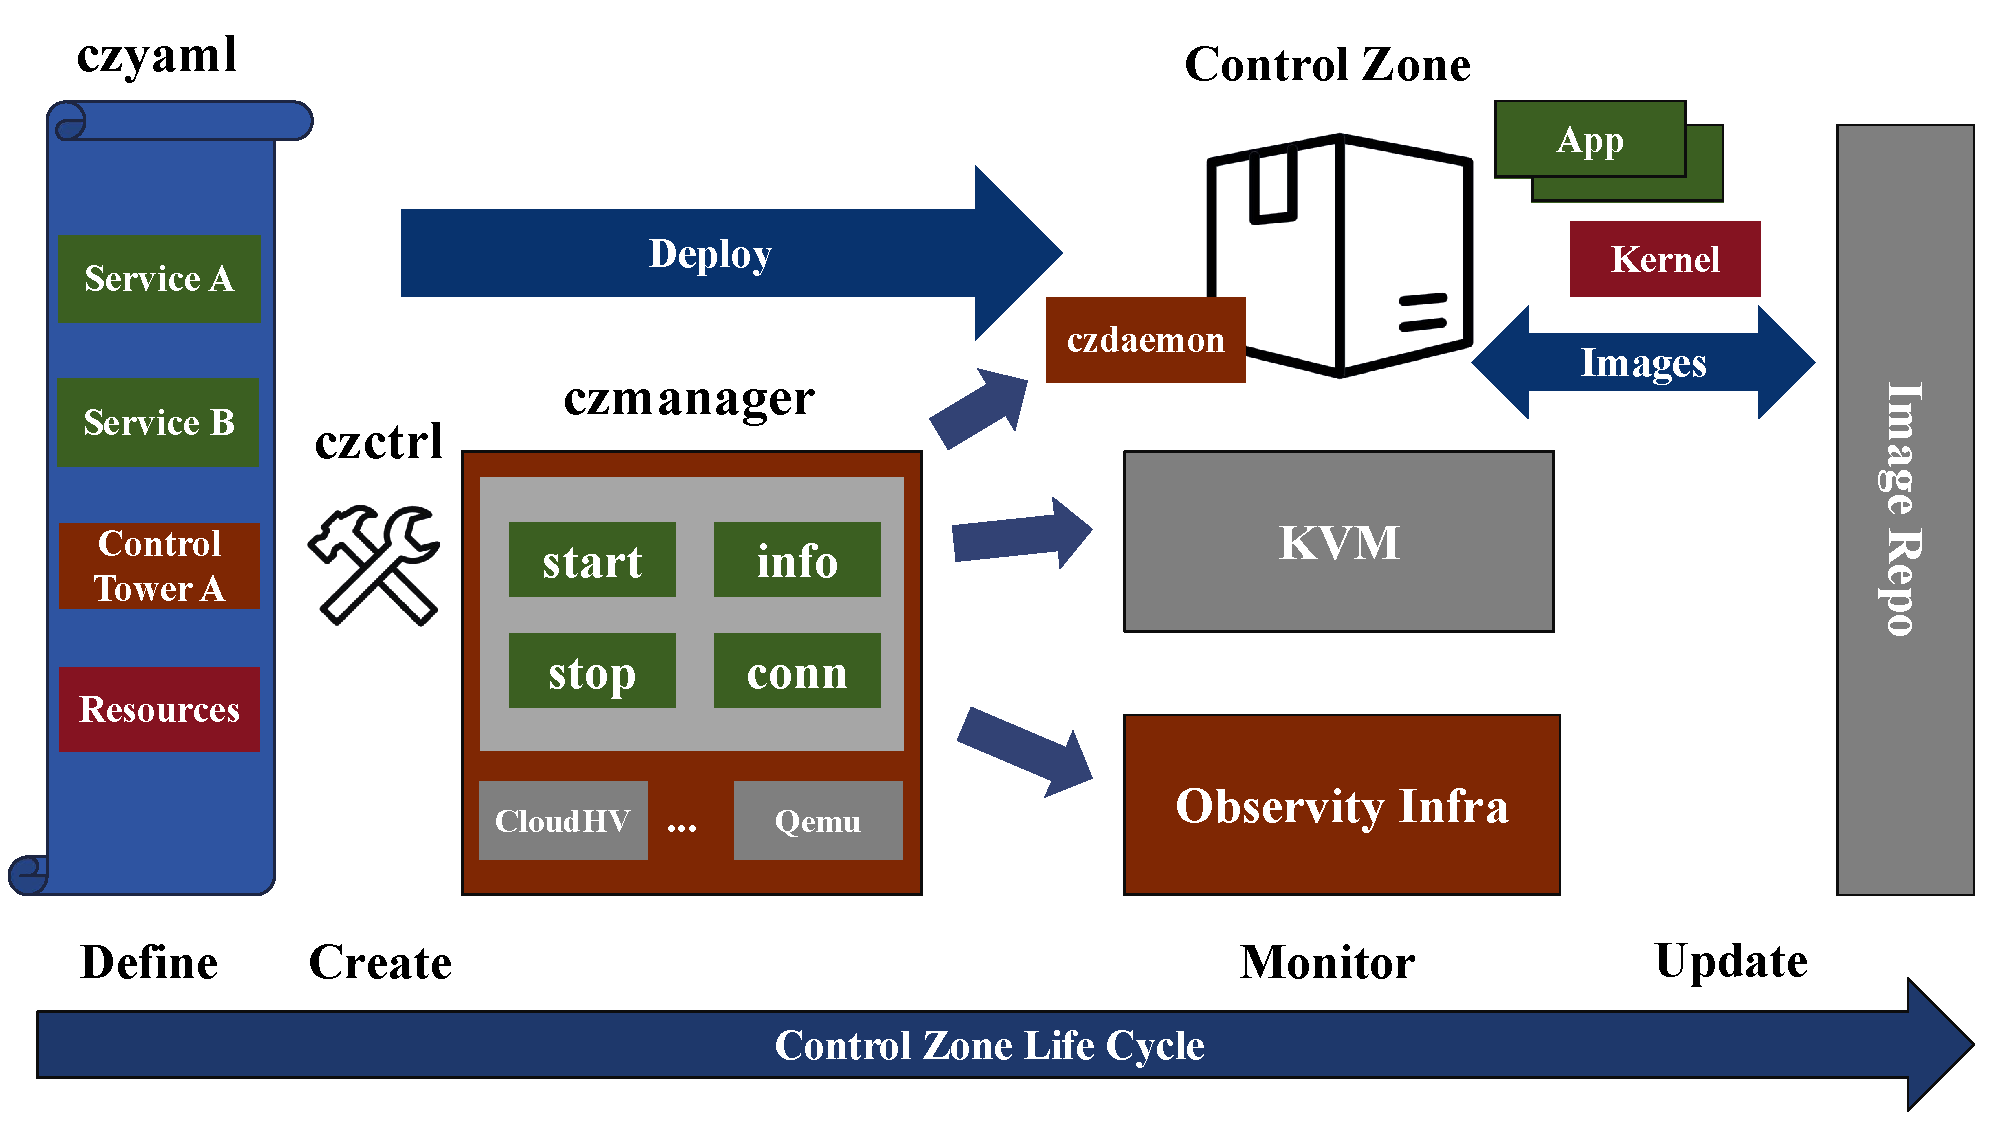
\includegraphics[width=0.9\textwidth]{cz_components}
    \bicaption{\quad Control Zone管理系统的组件架构}{\quad Architecture of the Control Zone management system}
    \label{fig:cz_components}
\end{figure}

\begin{itemize}

    \item \textbf{czyaml}:Control Zone定义。czyaml包含Meta、Guest、Resource三部分,其中Meta包含一些元数据,用以区分不同的Control Zone。Guest部分则用于声明运行环境,包括使用的系统、调度器及根文件系统。Resource部分用于声明隔离的资源,包括常见的CPU、Memory以及Intel RDT子系统中的LLC和内存带宽。

    \item \textbf{czmanager}:Control Zone管理。czmanager负责Control Zone的实际管理, 包括创建、查看、启动、暂停、更新以及清除等完善的生命周期管理。过程中czmanager主要负责维护Control Zone的状态,并协同底层虚拟机监视器实现最终的虚拟机管理。而在可观测性上,czmanager利用了虚拟机各层次的信息生成监控配置,并与可观测性基础设施协作以实现Control Zone的持续监控。资源管理上,czmanager主要与虚拟机监视器、Linux Resctrl及Cgroup子系统交互,根据czyaml中的定义实现Control Zone的资源隔离。

    \item \textbf{czdaemon}:Control Zone守护程序。czdaemon运行在每个Control Zone之中,在启动阶段主要用来信息获取与状态探测。而在启动完成之后,作为Control Zone内外沟通的桥梁,对外与czmanager交互,以接收命令,对内则直接与容器运行时交互,实现镜像及容器的管理。

    \item \textbf{czctrl}:用户命令行工具。czctrl是所有请求的入口,能够解析用户输入的命令并验证czyaml配置,随后再与czmanager交互以达成用户管理Control Zone和任务的目的。

    \item \textbf{Harbor镜像库}:容器镜像及其他OCI镜像的管理。Harbor是一个开源的企业级镜像管理服务,Control Zone中混部应用与Control Tower任务调度策略都以OCI容器镜像的形式保存在Harbor镜像库中。同时为方便其他资源的管理,预编译内核及根文件系统也同样以精简容器镜像的形式保存在镜像库中,并采用与容器镜像类似的形式管理。

\end{itemize}

\subsection{Control Zone管理过程}

% 要解决的问题,以及解决的问题的思路

% Control Zone Yaml
% Control Zone关键流程的执行过程
% - start
% - stop 
% - update
% - remove
% Control Zone容器的管理流程
% - add
% - delete
% Control Zone调度的流程
% - czctrl的资源限制
% - chsd的策略控制
% - sched ext的策略控制

Control Zone Yaml提供了丰富的配置选项,允许用户自定义沙箱的基本信息,并提供丰富的资源隔离配置。

\begin{itemize}
    \item \textbf{基础配置}:Control Zone基础配置如表~\ref{tab:cz_meta_config}所示,首先,在Guest环境上,Control Zone提供了Response、Throughput两种基本内核,用户可根据需要进行选择。而为加快启动速度,Control Zone默认不使用initramfs,并采用基于Alpine的轻量化rootfs。轻量化rootfs中仅包含基础的软件运行环境,用户也可根据需要进行修改。在应用管理上,Control Zone使用类似Pod Yaml的配置文件来描述混部任务的部署需求,其中Control Tower调度器与常规应用一样包含在配置文件中。

\begin{table}[H]
    \bicaption{\quad Control Zone 元配置选项}{\quad Control Zone meta configuration options}% caption
    \label{tab:cz_meta_config}
    \footnotesize% fontsize
    \setlength{\tabcolsep}{4pt}% column separation
    \renewcommand{\arraystretch}{1.25}% row space 
    \centering
    \begin{tabular}{lc}
        \hline
        %\multicolumn{num_of_cols_to_merge}{alignment}{contents} \\
        %\cline{i-j}% partial hline from column i to column j
        配置 & 说明\\
        \hline
        name & Control Zone名称 \\
        workdir & Control Zone工作目录,存放日志及其他配置 \\
        share\_folder(可选) & 额外共享给Control Zone的目录 \\
        label & 标签,数个key-value对 \\
        vrun & 虚拟机监视器,可额外选Qemu、Libvirtd \\
        initramfs(可选) & 初始化内存文件系统 \\
        rootfs(可选) & Control Zone使用的根文件系统,从镜像存储拉取\\
        kcmdline(可选) & 内核的运行命令 \\
        apps(可选) & App容器配置 \\
        \hline
    \end{tabular}
\end{table}

    \item \textbf{资源配置}:KVM虚拟机是一种特殊的进程,Control Zone在创建虚拟机的过程中,会为vCPU及emulator线程创建Cgroup与Resctrl Monitor Group来方便进行资源管理。具体的资源配置选项如表~\ref{tab:cz_cgroup_config}所示。首先,可基于Cgroup配置vCPU线程的相关资源,如CPU亲和性与CPU时间片配置。其次,也可通过Resctrl子系统为整个虚拟机线程组配置LLC掩码,来进行Cache资源的隔离。

\begin{table}[H]
    \bicaption{\quad Control Zone资源配置选项}{\quad Control Zone resource configuration options}% caption
    \label{tab:cz_cgroup_config}
    \footnotesize% fontsize
    \setlength{\tabcolsep}{30pt}% column separation
    \renewcommand{\arraystretch}{1.25}% row space 
    \centering
    \begin{tabular}{lc}
        \hline
        %\multicolumn{num_of_cols_to_merge}{alignment}{contents} \\
        %\cline{i-j}% partial hline from column i to column j
        配置 & 说明\\
        \hline
        cpu.max & 最大CPU使用限制 \\
        cpu.max.burst & 最大突发CPU使用限制 \\
        cpuset.cpus & CPU亲和性 \\
        cpuset.mems & 内存节点亲和性 \\
        llc mask& 可用LLC掩码 \\
        \hline
    \end{tabular}
\end{table}

    \item \textbf{Hypervisor配置}:虚拟机硬件通常由Hypervisor模拟,其中如virtio设备等在模拟设备后端驱动上提供了丰富的配置选项。通过Hypervisor提供的调控接口,可进一步在设备上进行资源隔离的配置。具体配置如表~\ref{tab:cz_hv_config}所示。首先,对于CPU资源,可配置虚拟机所能使用的CPU feature。对于virtio网络设备和块设备,则可在读写速度上进行配置。

\begin{table}[H]
    \bicaption{\quad Control Zone 虚拟机监视器配置选项}{\quad Control Zone hypervisor configuration}% caption
    \label{tab:cz_hv_config}
    \footnotesize% fontsize
    \setlength{\tabcolsep}{30pt}% column separation
    \renewcommand{\arraystretch}{1.25}% row space 
    \centering
    \begin{tabular}{lc}
        \hline
        %\multicolumn{num_of_cols_to_merge}{alignment}{contents} \\
        %\cline{i-j}% partial hline from column i to column j
        配置 & 说明\\
        \hline
        cpu features& vCPU可用的特性\\
        bw\_size & 设备带宽大小(byte/s)\\
        bw\_one\_time\_burst & 设备突发带宽大小(byte/s)\\
        bw\_refill\_time & 设备带宽恢复时间(ms)\\
        ops\_size & 设备操作速度(op/s)\\
        ops\_one\_time\_burst & 设备突发操作速度(op/s)\\
        ops\_refill\_time & 设备操作速度恢复时间(ms)\\
        \hline
    \end{tabular}
\end{table}

\end{itemize}

czctrl提供了create、start、stop、remove、update五种操作来管理Control Zone的生命周期。Control Zone的状态变化如图~\ref{fig:cz_state}所示,其中sync过程由czdaemon完成,并同步给czmanager。对于不能直接达到的状态,czmanager会试图多次切换状态以满足目标。对于无法达到的状态,czmanager会提示操作非法,并终止正在进行的操作。update操作并未在图中,其过程由多个已有的其他操作组成。取决于更新的内容,update具体的操作也有所不同,如对内核的修改将使得Control Zone重新启动,而仅修改CPU时间片大小则不会影响Control Zone的运行状态。

\begin{figure}[!htbp]
    \centering
    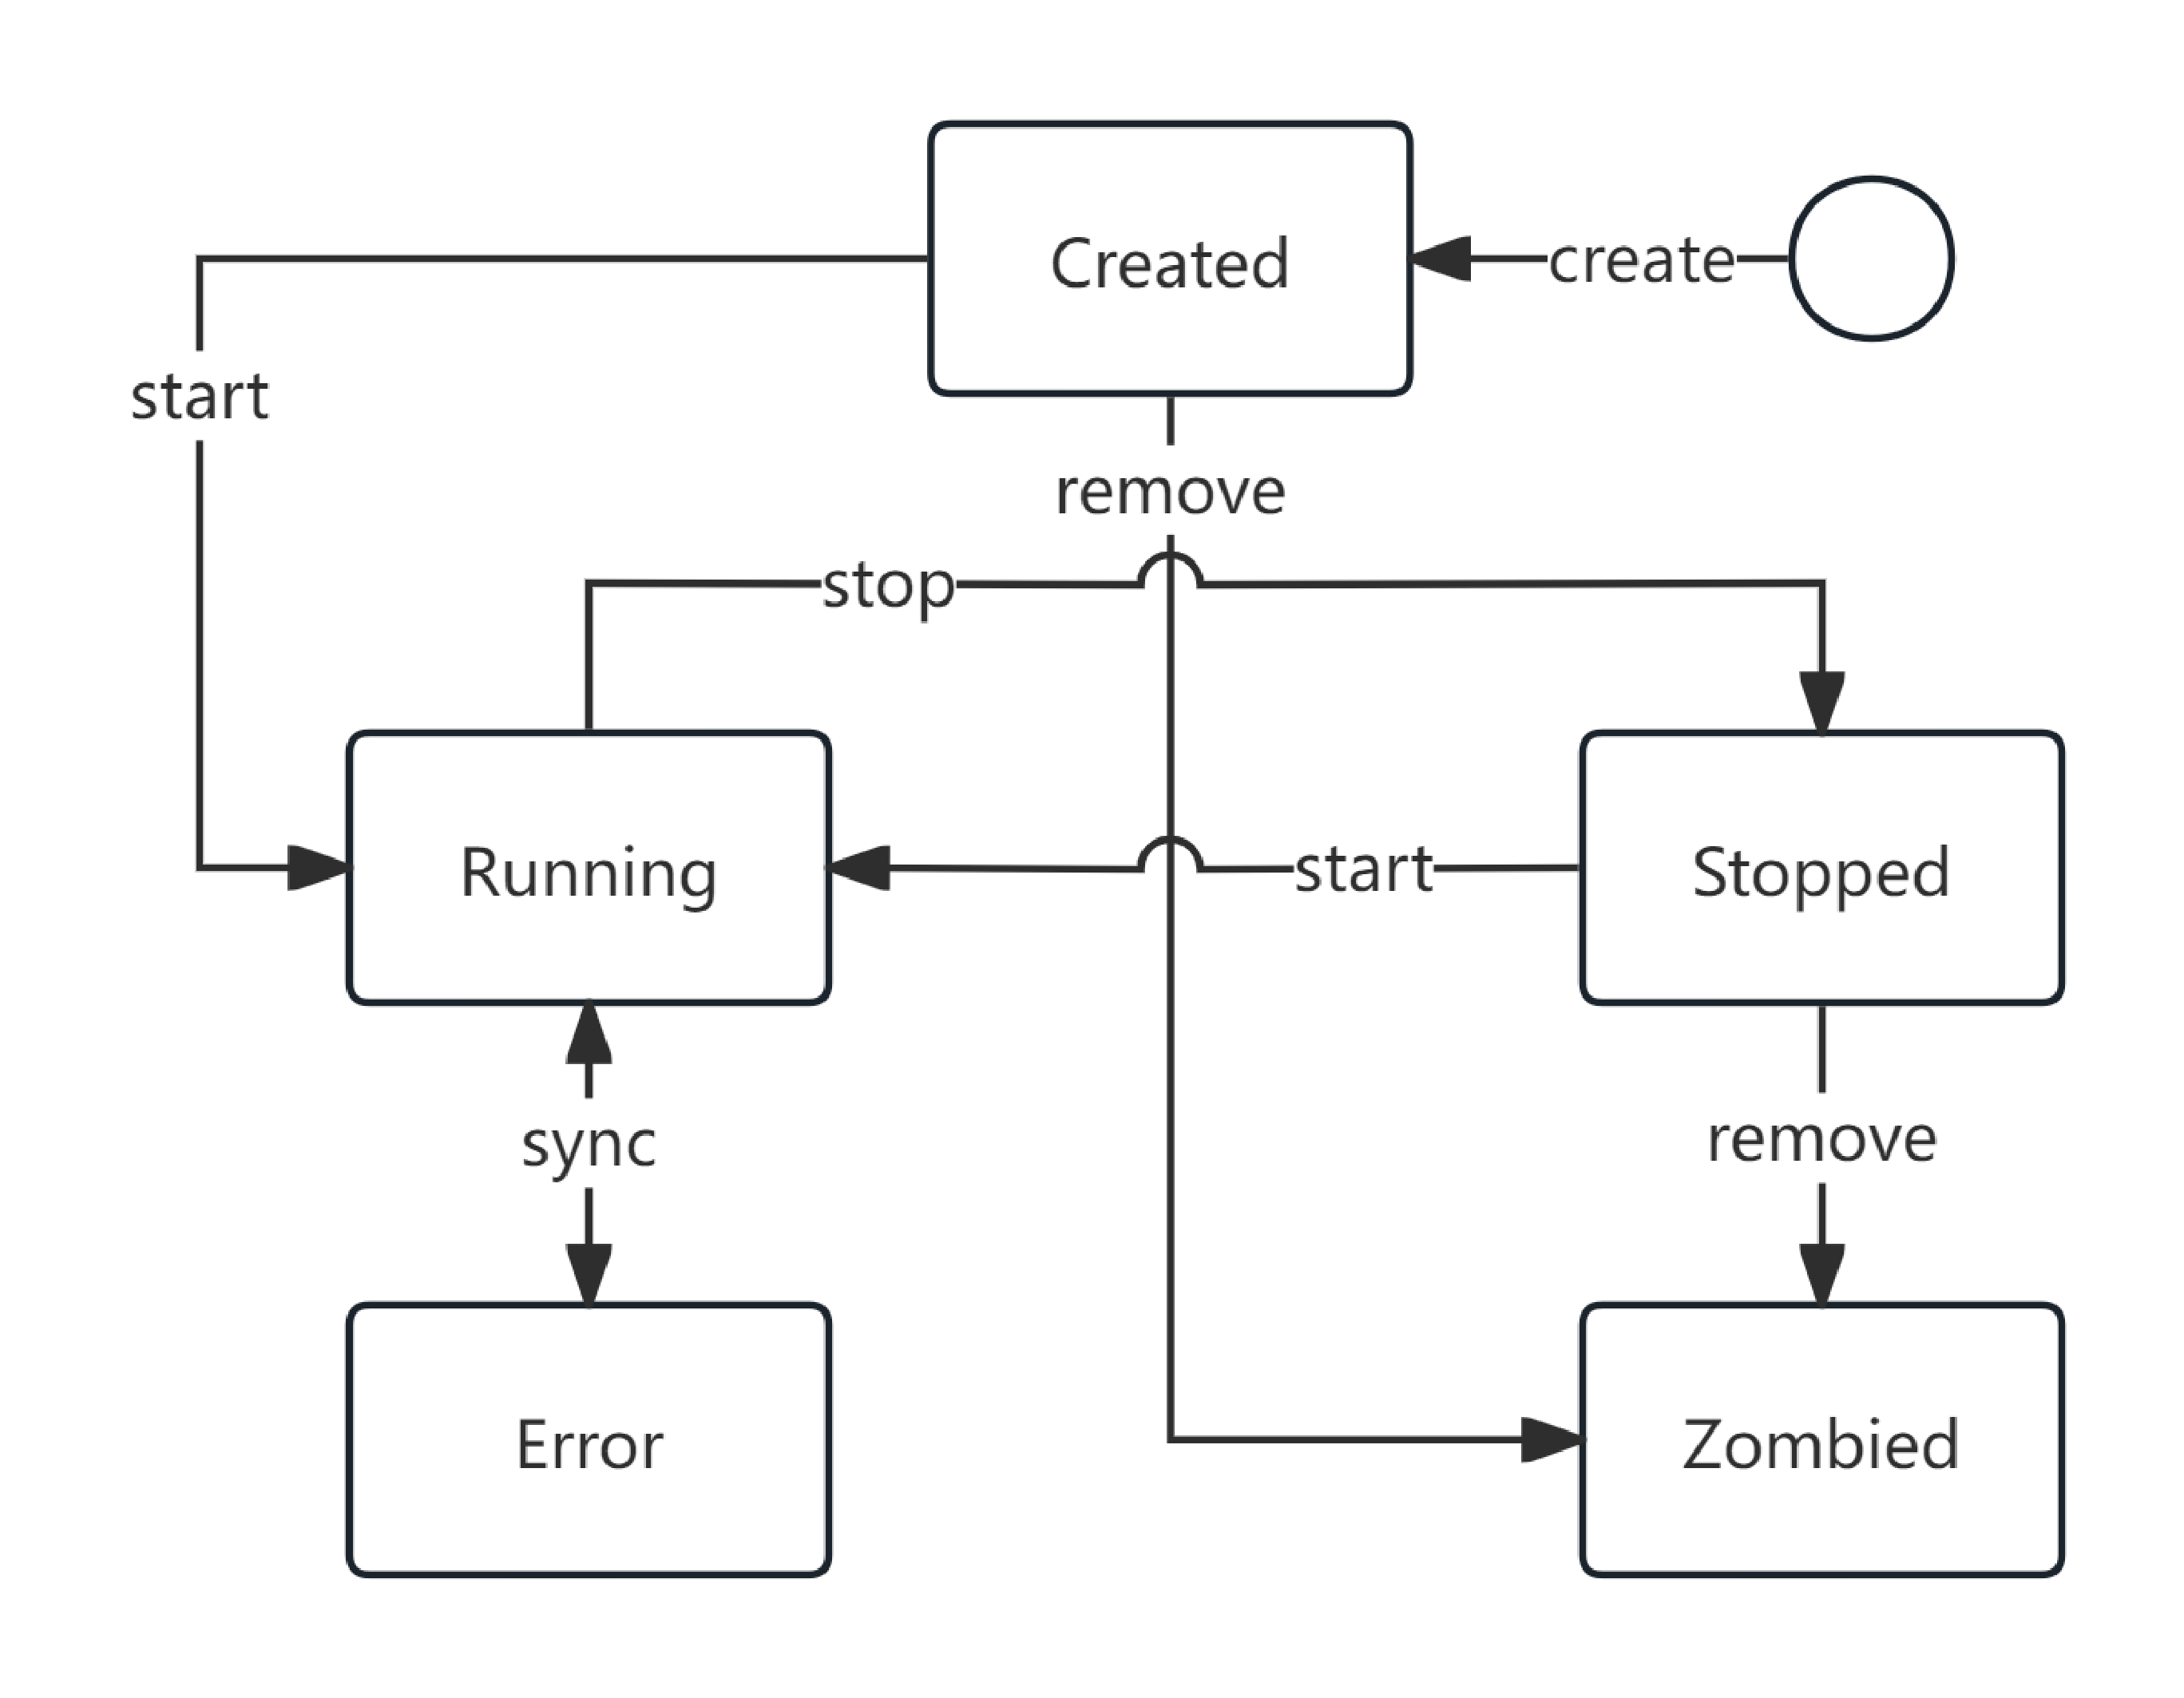
\includegraphics[width=0.5\textwidth]{cz_state}
    \bicaption{\quad Control Zone状态迁移设计}{\quad Control Zone state transition design}
    \label{fig:cz_state}
\end{figure}

Control Zone的创建过程如图~\ref{fig:cz_create}所示。过程中首先进行配置的合法性监测,创建过程中的检测主要判断资源是否重复分配,如对于cpuset,czmanager会检查全局的cpu mask来判断cpuset的设置是否合法。随后进行工作目录的创建,用来单独保存每个Control Zone的关键数据,如根文件系统等。创建过程仅为虚拟机的启动做好准备,而并不会启动虚拟机,相当于为虚拟机的启动预留了资源。

\begin{figure}[H]
    \centering
    \begin{subfigure}[b]{0.42\textwidth}
        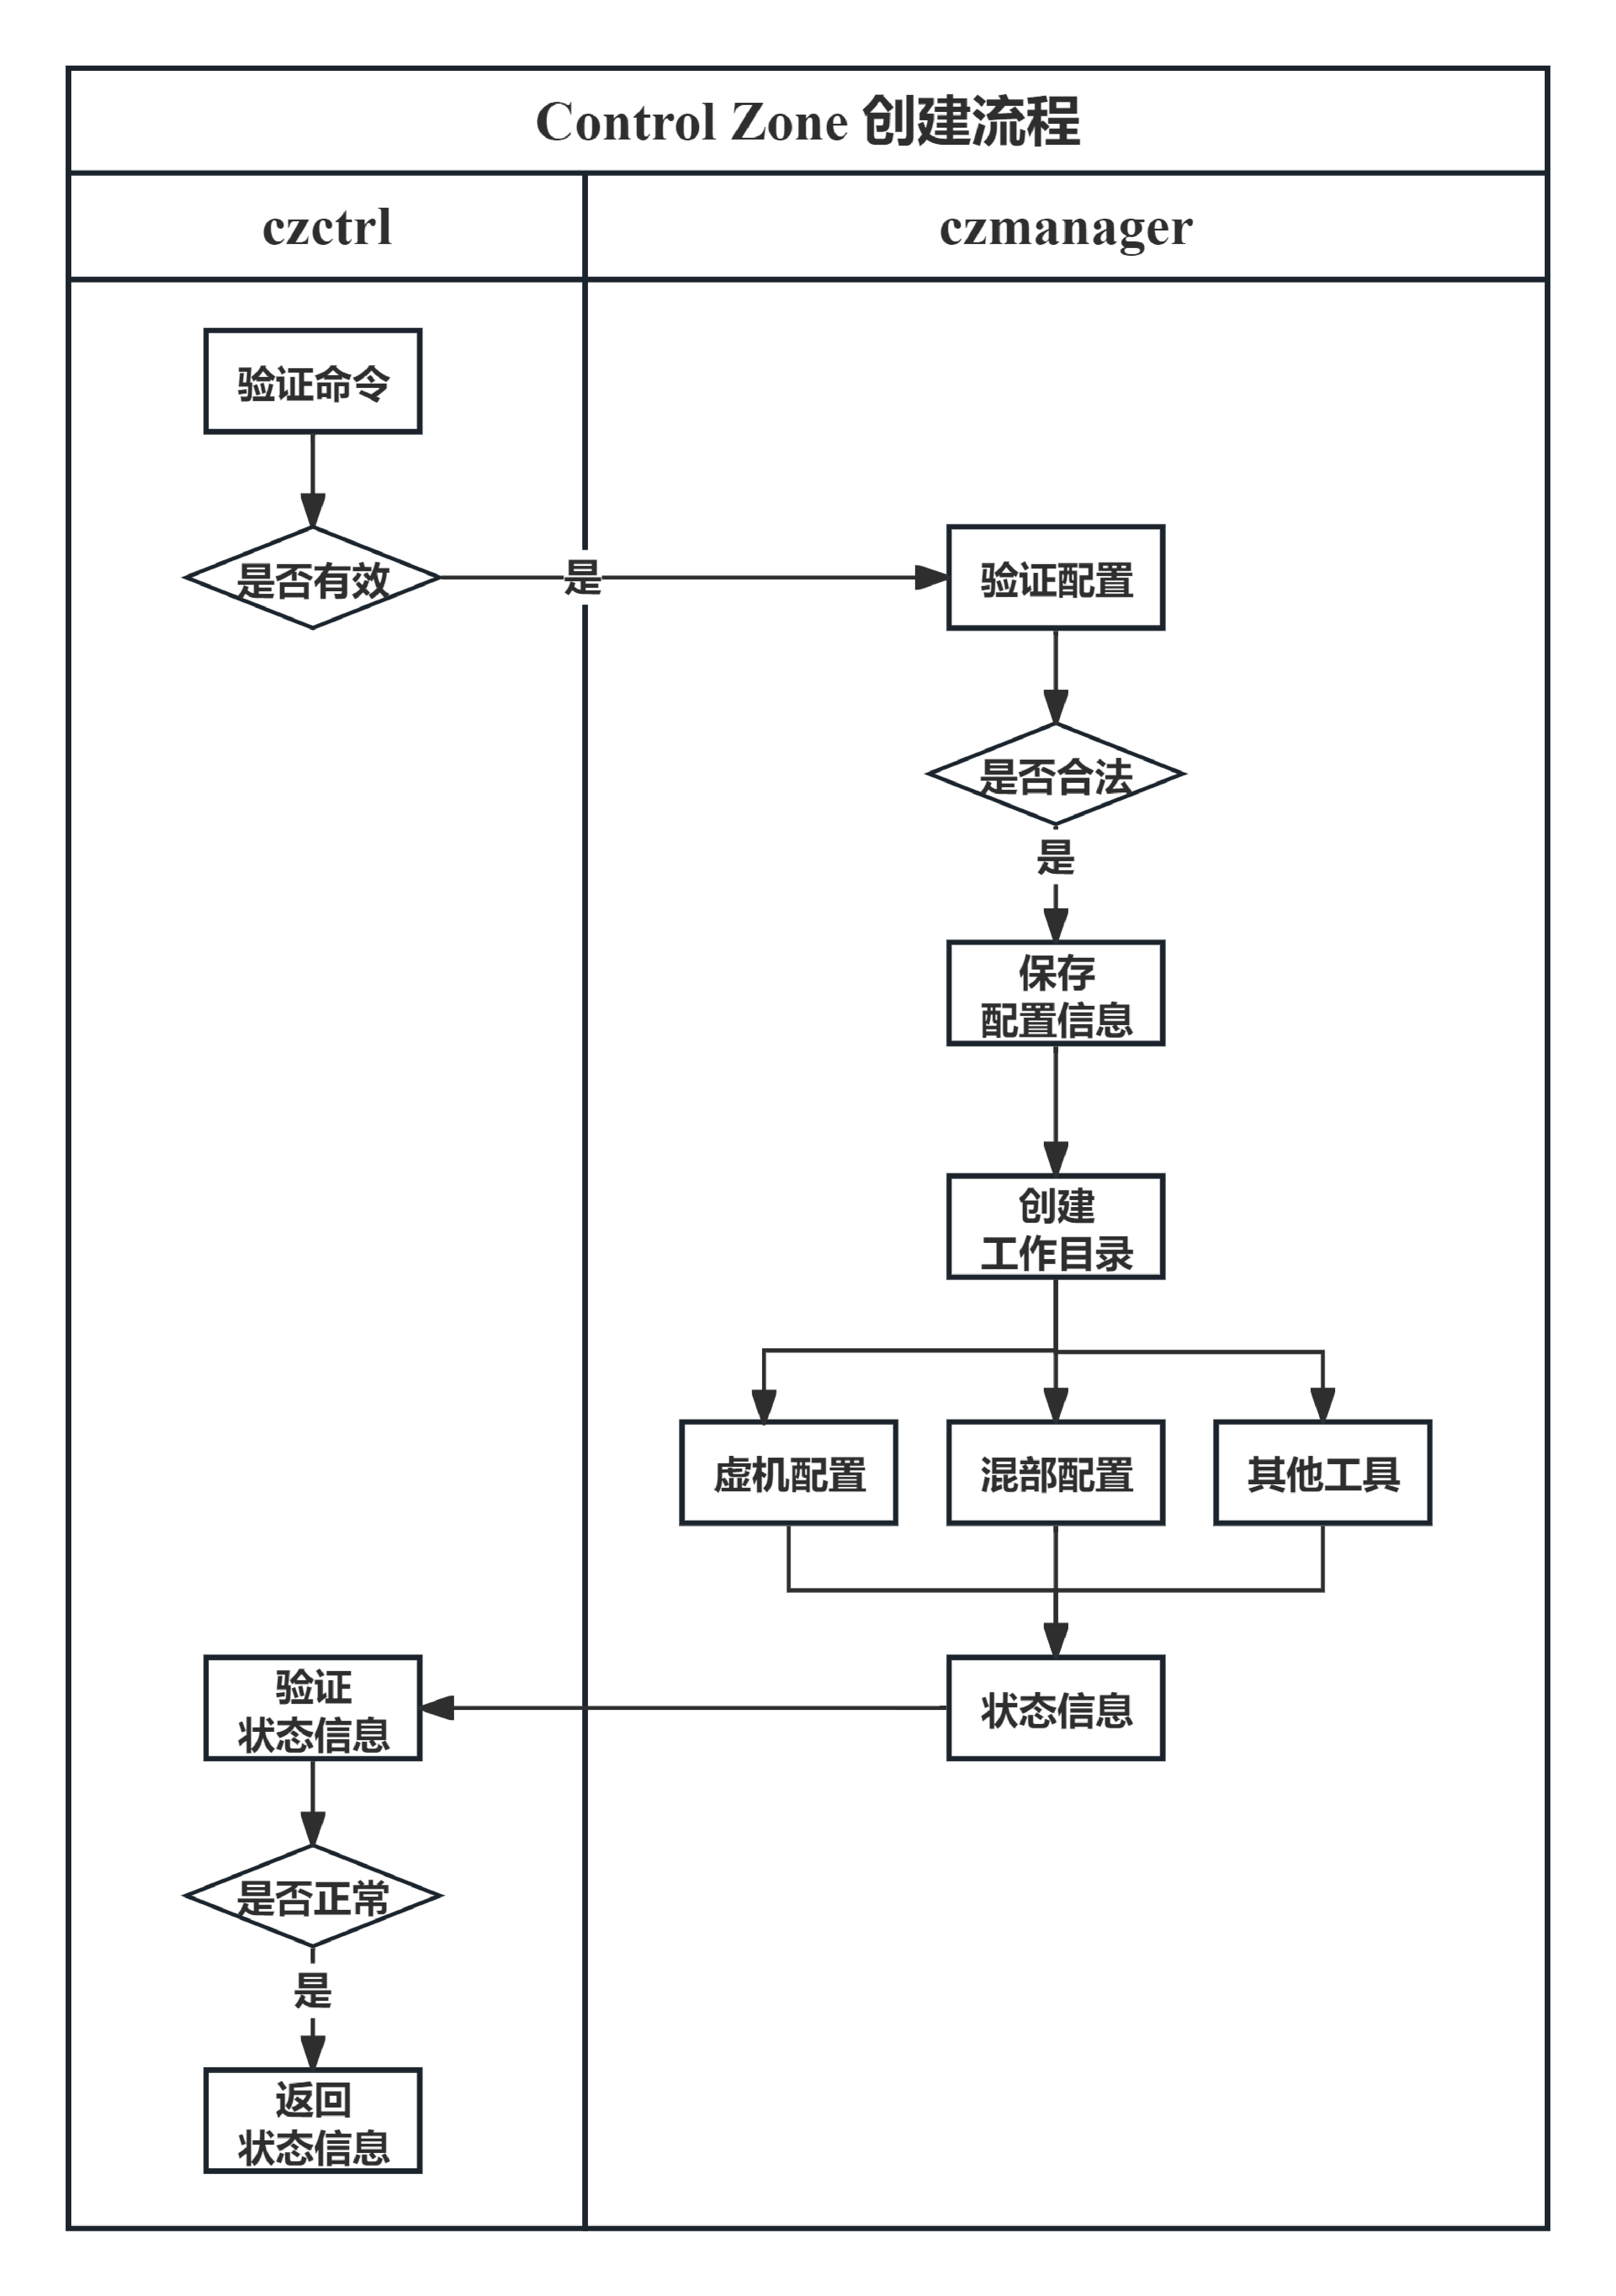
\includegraphics[width=\textwidth]{cz_create}
        \caption{\quad Control Zone创建过程}
        \label{fig:cz_create}
    \end{subfigure}
    \hfill
    \begin{subfigure}[b]{0.56\textwidth}
        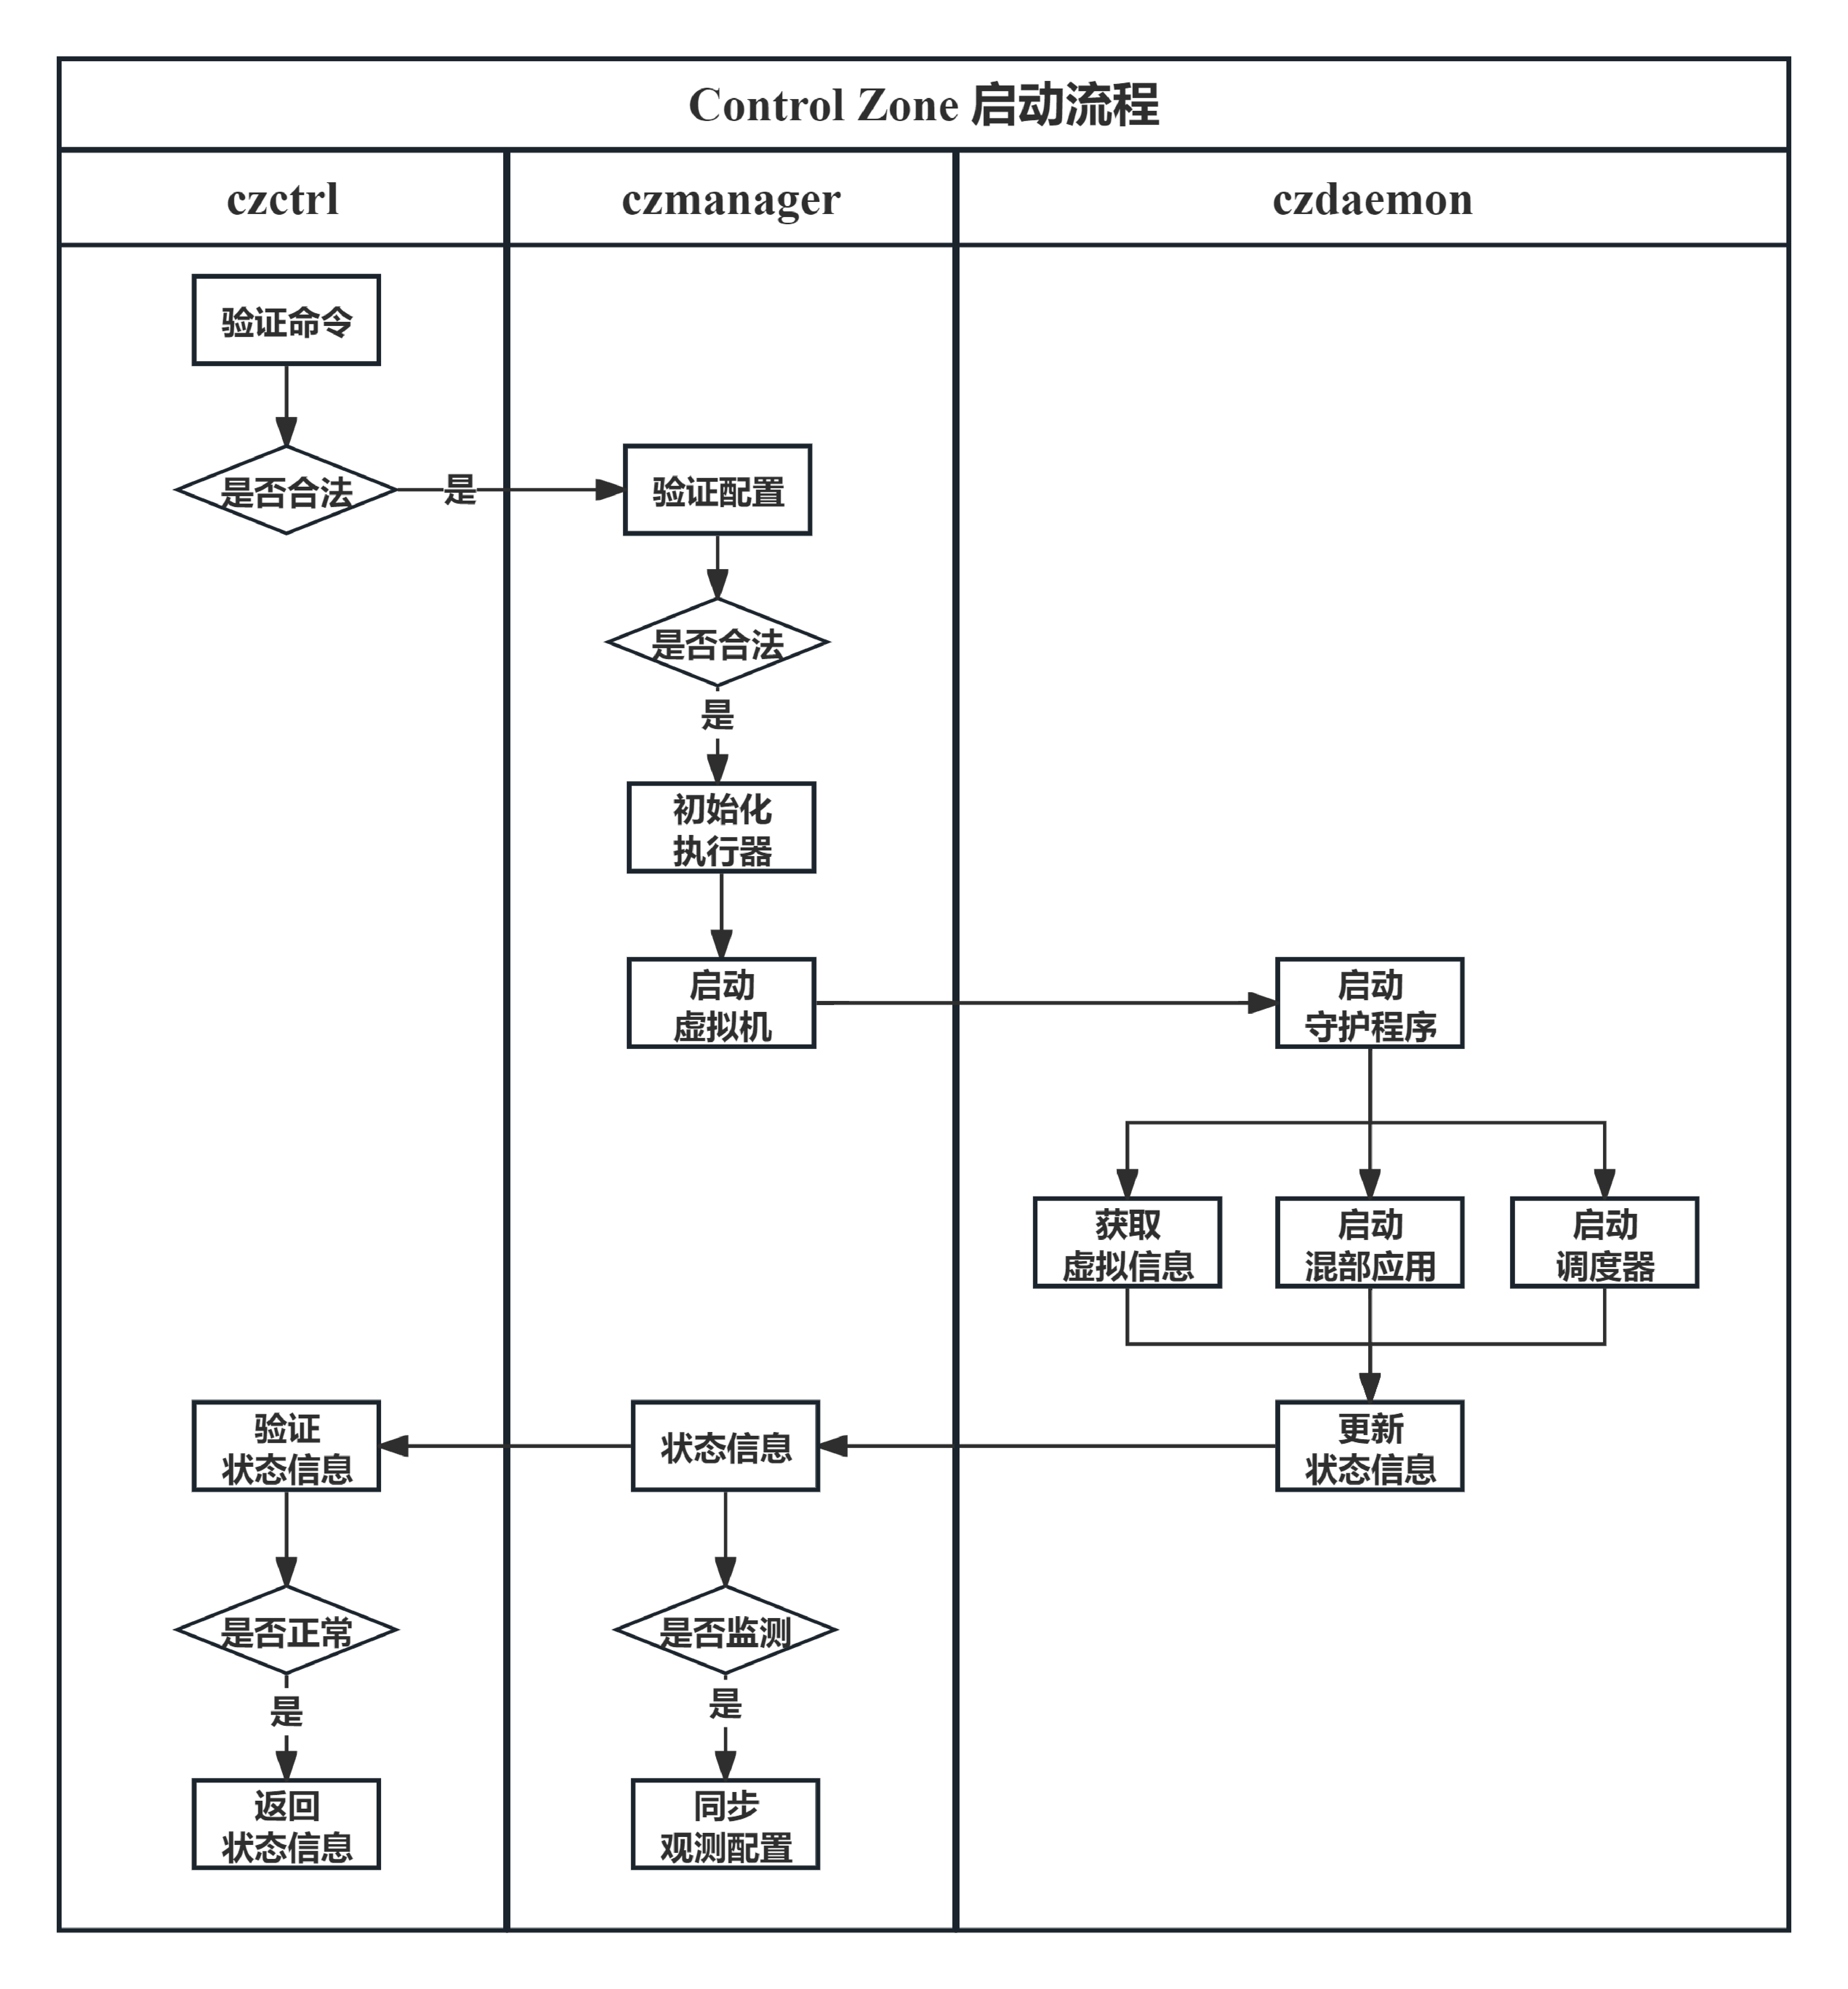
\includegraphics[width=\linewidth]{cz_start}
        \caption{\quad Control Zone启动过程}
        \label{fig:cz_start}
    \end{subfigure}
\bicaption{\quad Control Zone创建与启动过程}{\quad Control Zone creation and startup process }
\label{fig:cz_create_start}
\end{figure}

Control Zone的启动过程如图~\ref{fig:cz_start}所示。过程中首先进行配置的合法性监测,如判断状态迁移是否合法、验证资源是否重复分配。对于一个已经创建的Control Zone,其预留的资源并不是严格进行保护的,因此在启动时其资源可能已经被占用,此时需要涉及重新更新Control Zone的资源配置。而在一切准备就绪以后,czmanager会按照配置要求,调用虚拟机监视器来启动虚拟机。而在虚拟机启动完毕之后,czdaemon会检测是否有已经提交的任务,并依次在后台进行执行,随后通知czmanager虚拟机状态的变化。czmanager在收到信号之后,Control Zone的启动过程就完成,而随后czmanager会根据配置来选择为Control Zone同步观测配置。

Control Zone的关闭过程如图~\ref{fig:cz_stop}所示。考虑关闭之后存在重新启动的可能,因此沙箱采用了较为保守的关闭策略。关闭过程中需要czmanager与czdaemon协同合作。在验证配置之后,czmanager首先会通知czdaemon进行关闭处理。而czdaemon在接收到关闭信号之后,会对当前系统的状态进行保存,包含必要的信息、混部应用状态等,随后终止混部应用的运行并通知czmanager。收到通知后czmanager才会调用执行器关闭虚拟机,并在必要时通知可观测性基础停止监测。Control Zone在停止之后仍会保留部分资源分配信息,便于后续重新启动。

\begin{figure}[H]
    \centering
    \begin{subfigure}[b]{0.46\textwidth}
        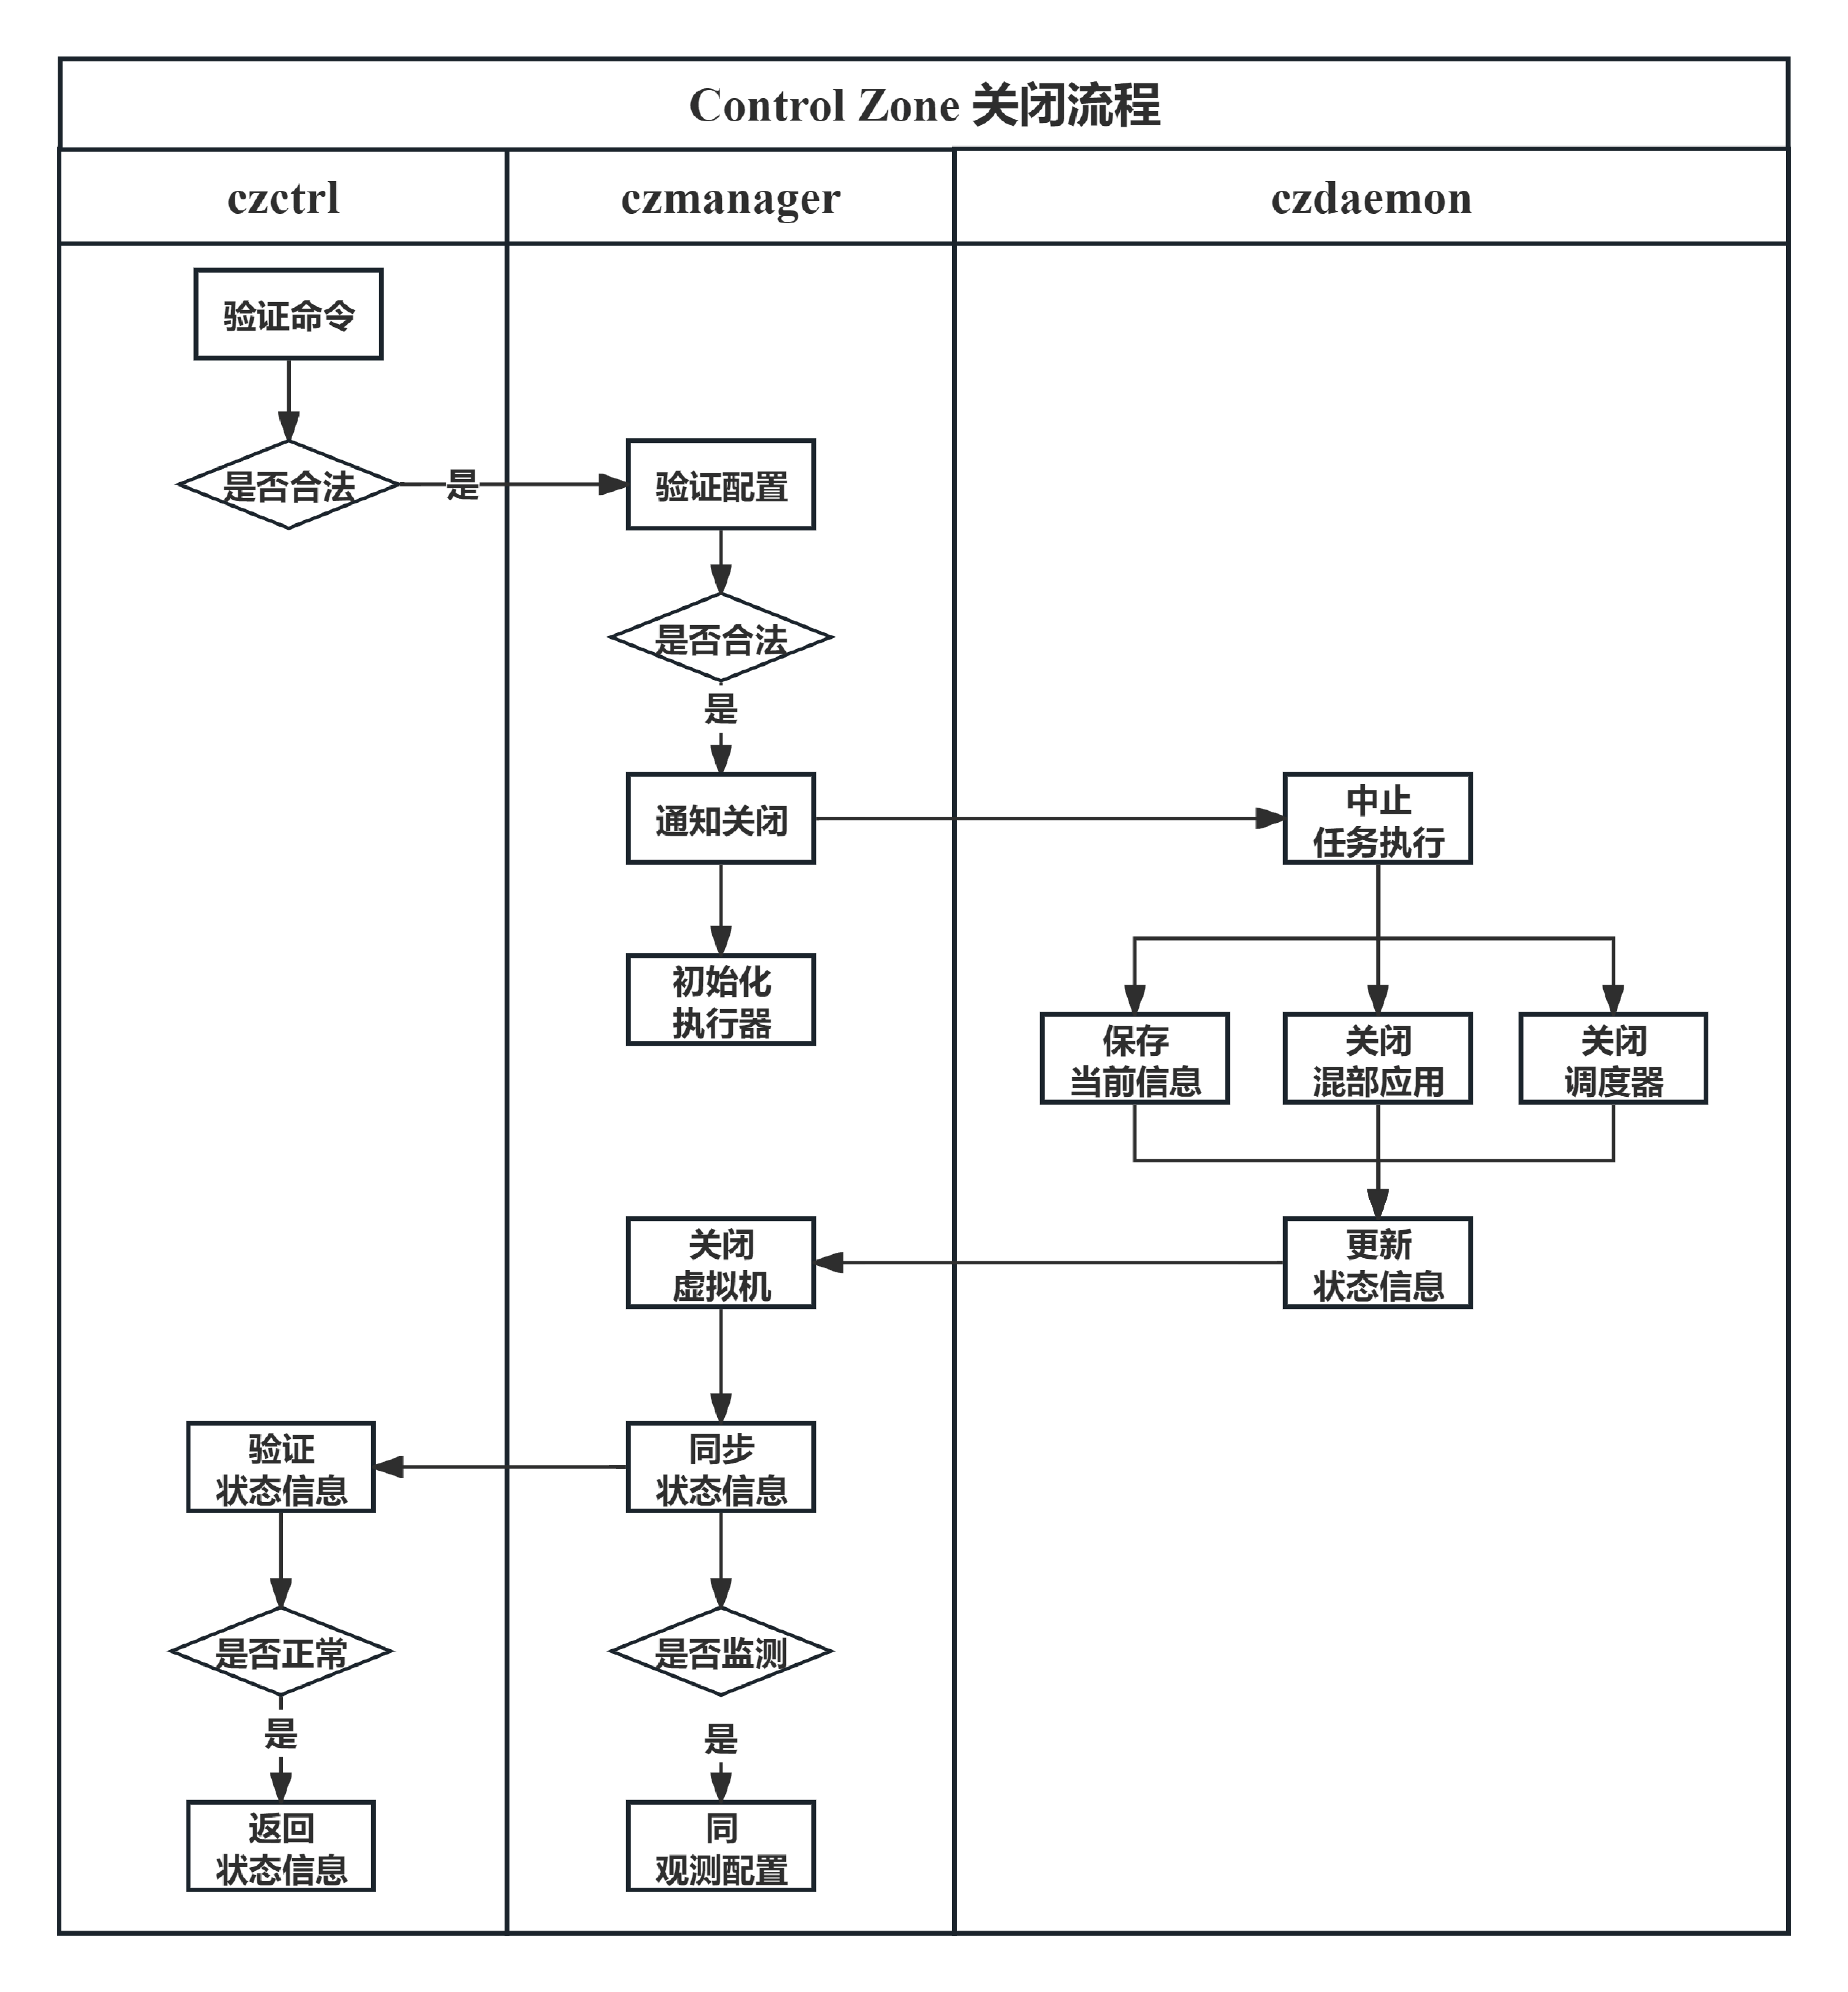
\includegraphics[width=\textwidth]{cz_stop}
        \caption{\quad Control Zone关闭过程}
        \label{fig:cz_stop}
    \end{subfigure}
    \hfill
    \begin{subfigure}[b]{0.53\textwidth}
        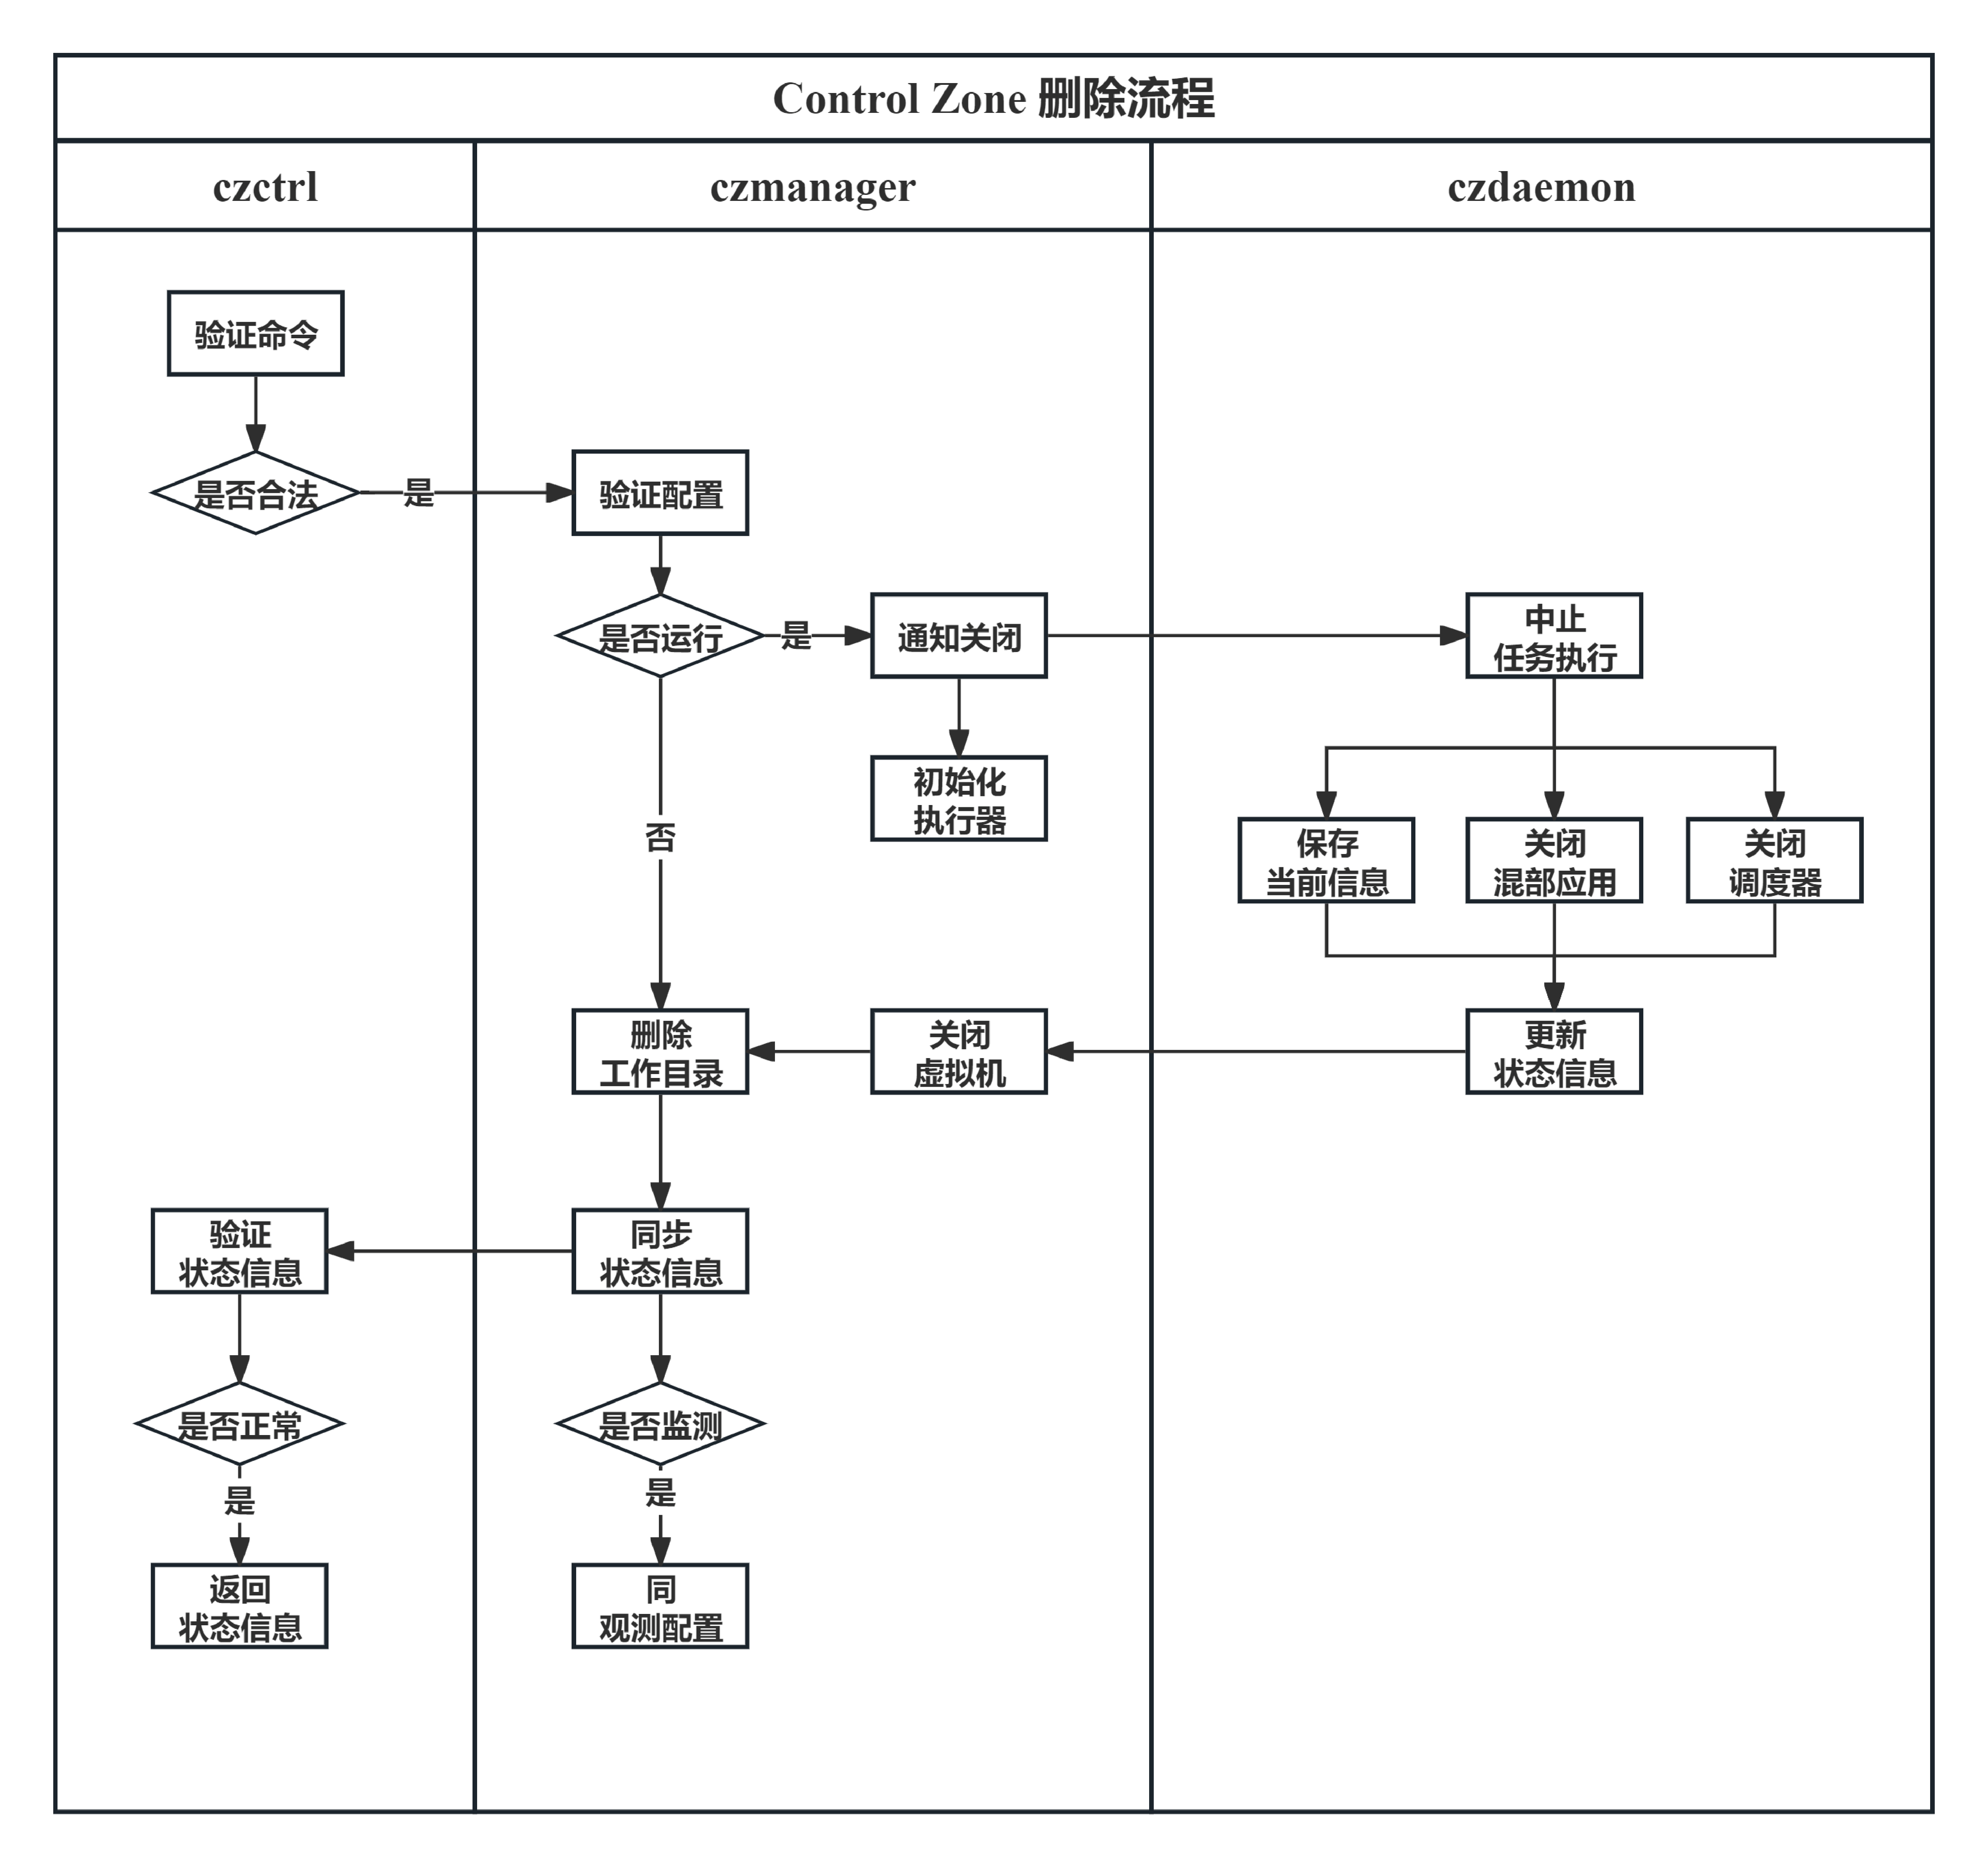
\includegraphics[width=\textwidth]{cz_remove}
        \caption{\quad Control Zone删除过程}
        \label{fig:cz_remove}
    \end{subfigure}
\bicaption{\quad Control Zone关闭与删除过程}{\quad Control Zone shutdown and deletion process }
\label{fig:cz_stop_delete}
\end{figure}

Control Zone的删除过程如图~\ref{fig:cz_remove}所示。通常只有已经停止的Control Zone能够被删除。为简化操作,当Control Zone为其他状态时,此时进行删除操作时会首先将Control Zone的状态转化为停止状态,再进行删除操作。Control Zone的除了工作目录的销毁外,还会回收已经分配的资源。

Control Zone的更新过程如图~\ref{fig:cz_update}所示。Control Zone Yaml中的绝大部分字段都允许被更新。部分配置的更新在Control Zone运行中完成,如修改cgroup或resctrl等字段中的内容。czmanager发现这部分字段修改时,会重新修改资源隔离配置,并调用各个资源管理接口来进行实施。而部分字段则会涉及到Control Zone的重新启动,如对Guest中的内核、根文件系统等字段进行修改。czmanager检测到这些字段发生修改后,首先会关闭虚拟机,随后在工作目录中更新配置所要求的内容,最后再启动虚拟机。通常更新完毕后,由于虚拟机进程的变化,可观测配置有可能过时,因此czmanager还会同步配置给可观测性基础设施。

本文在Control Zone管理器的各个组件实现中,使用Rust语言编写了约3500行代码。同时项目被组织为多个crate,能够方便组件之间共享公共代码,并未后续引入新特性和增量开发提供便利。

\begin{figure}[H]
    \centering
    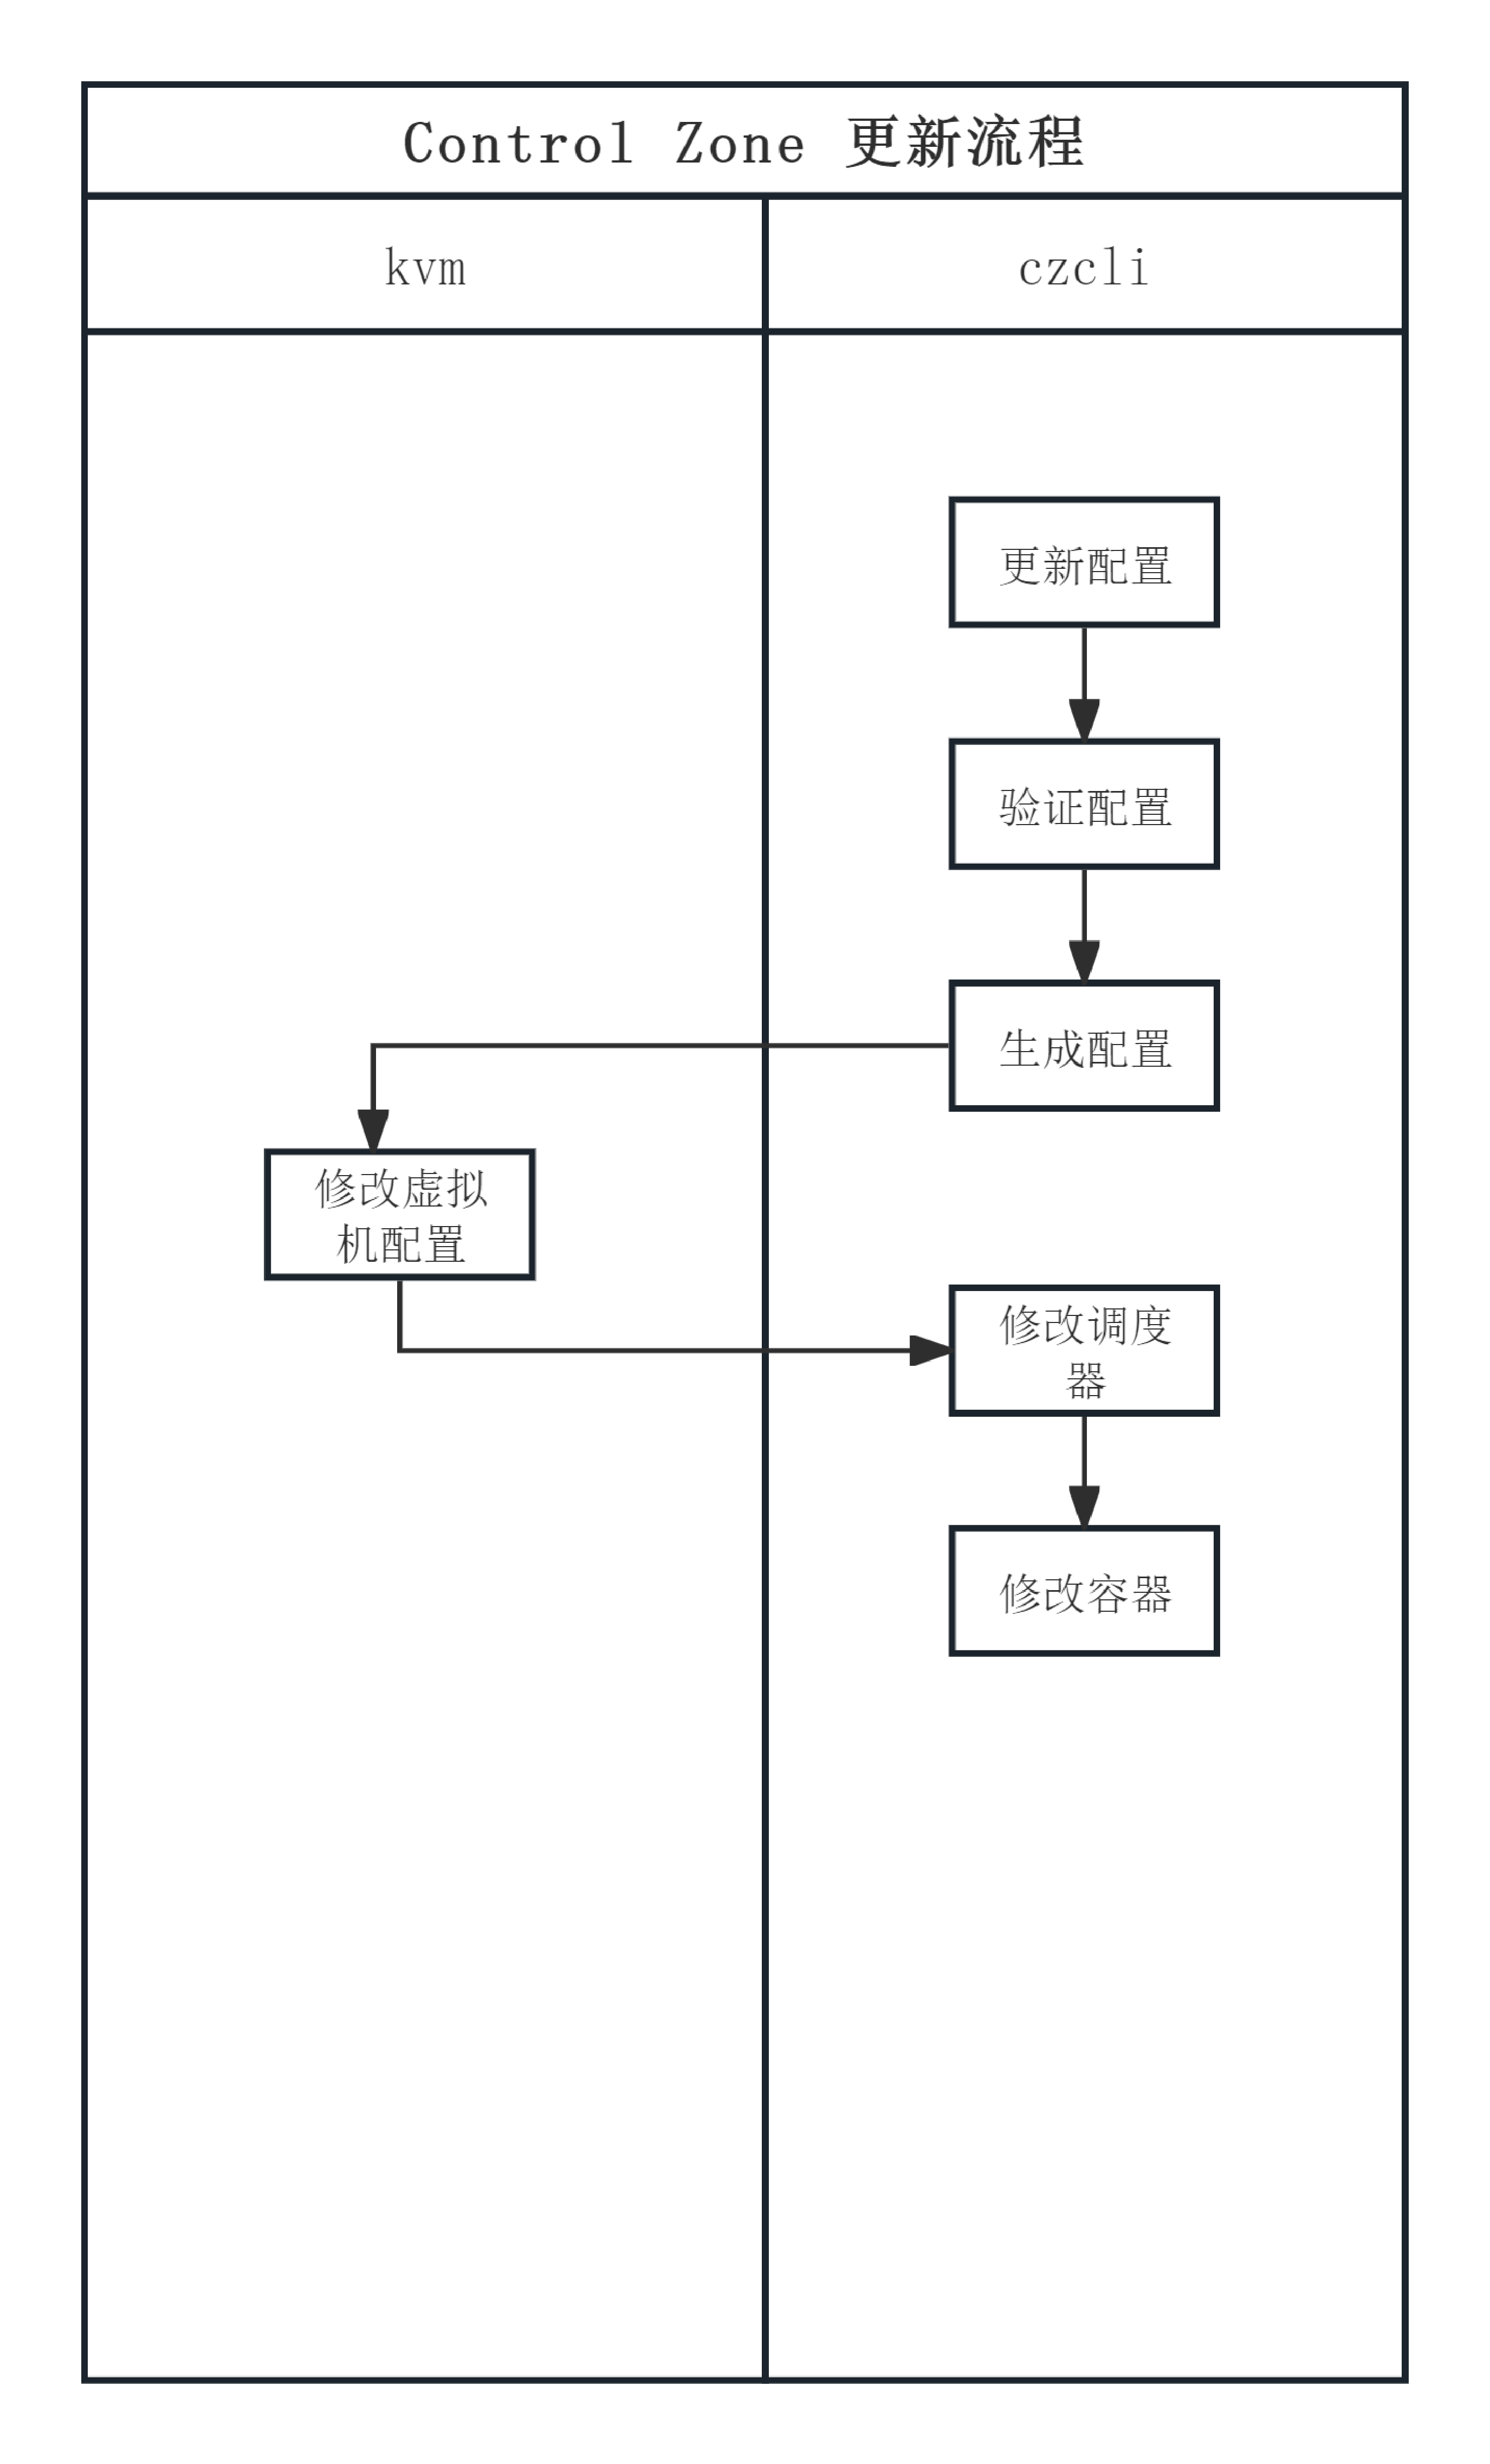
\includegraphics[width=0.6\textwidth]{cz_update}
    \bicaption{\quad Control Zone更新过程}{\quad Control Zone update process }
    \label{fig:cz_update}
\end{figure}

\section{实验设计与分析}

\subsection{实验环境}

实验环境由两台服务器构成,服务器硬件信息如表~\ref{tab:sandbox_exp_env}所示。在CPU资源上,每台服务器上包含有两个Socket,单台总计80个物理核心,划分为4个Numa Node。同时,CPU均开启超线程,并使能Intel RDT。在网络资源上,服务网卡支持SRIOV技术,能为有网络性能需求的虚拟机提供硬件直通支持。

\begin{table}[H]
    \bicaption{\quad 沙箱实验服务器硬件参数}{\quad Information about server hardware for sandbox experiments}% caption
    \label{tab:sandbox_exp_env}
    \footnotesize% fontsize
    \setlength{\tabcolsep}{4pt}% column separation
    \renewcommand{\arraystretch}{1.25}% row space 
    \centering
    \begin{tabular}{lc}
        \hline
        硬件资源 & 硬件信息 \\
        \hline
        CPU & Intel Xeon Gold 6148 (40 cores) * 2 \\
        Processor Core Frequency & 2.4GHz,Turbo 3.7 GHz \\
        L1 Caches & 32KB,  8-way set associative, split D/I \\
        L2 Caches & 1024KB, 16-way set associative \\
        L3 Caches & 28160KB, 11-way set associative \\
        Main Memory & 32GB * 8, 2666MHz DDR4 \\
        NIC & Intel Corporation Ethernet Connection X722 for 10GbE SFP+(10Gbit) \\
        \hline
    \end{tabular}
\end{table}

每台服务器的系统软件环境如表~\ref{tab:system_env}所示。在操作系统上,实验中选择使用较常见的Ubuntu22.04LTS。在虚拟机监视器以及相关环境上,Libvirt与Qemu采用Ubuntu22.04所支持的稳定版,CloudHyeprvirsor则采用v38.0-150编译版。

\begin{table}[H]
    \bicaption{\quad 沙箱实验服务器系统环境}{\quad Information about server system for sandbox experiments}% caption
    \label{tab:system_env}
    \footnotesize% fontsize
    \setlength{\tabcolsep}{30pt}% column separation
    \renewcommand{\arraystretch}{1.25}% row space 
    \centering
    \begin{tabular}{lc}
        \hline
        软件类型 & 软件信息 \\
        \hline
        系统 & Ubuntu 22.04.3 LTS  \\
        内核 & 5.15.0-79-generic \\
        虚拟机监视器 & cloud-hypervisor v38.0-150 \\
                   & QEMU emulator version 6.2.0 \\
        其他        & libvirtd 8.0.0 \\
        \hline
    \end{tabular}
\end{table}

服务器均部署了Black Box观测系统,并在主服务器上额外部署了Harbor镜像库。实验中所有的组件都以容器的形式运行,并较轻量的Podman作为服务器中的容器运行时。Podman相较Docker更加轻量,且不存在Docker、Containerd等后台驻留服务,能够提供较纯净的环境。而为避免可观测性基础设施对其他应用的影响,各组件都配置了CPU亲和性并限制在固定的CPU、NUMA上运行。

\subsection{Control Zone启动开销}

启动开销为从虚拟机监视器启动到系统引导至init的时间。在虚拟机监视器上,选择CloudHyperviosr与Qemu。在内核上,选择Alpine Virt内核、Control Zone内核、CloudHypervirsor默认内核及Firecracker默认内核。Alpine Virt内核为社区的标准虚拟机内核,保留了对于众多设备的支持。CloudHyeprvirsor、Firecracker默认内核以轻量为目标,相较于Alpine Virt内核去除了大量驱动,几乎只支持virtio设备。CloudHypervisor默认内核还额外使能了PCI以支持SRIOV。实验中虚拟机配置均为1 CPU、512 MB内存,且使用virtio pci设备。为使得实验结果具备可比较性,使能了Firecracker默认内核的PCI支持。

\begin{figure}[H]
    \centering
    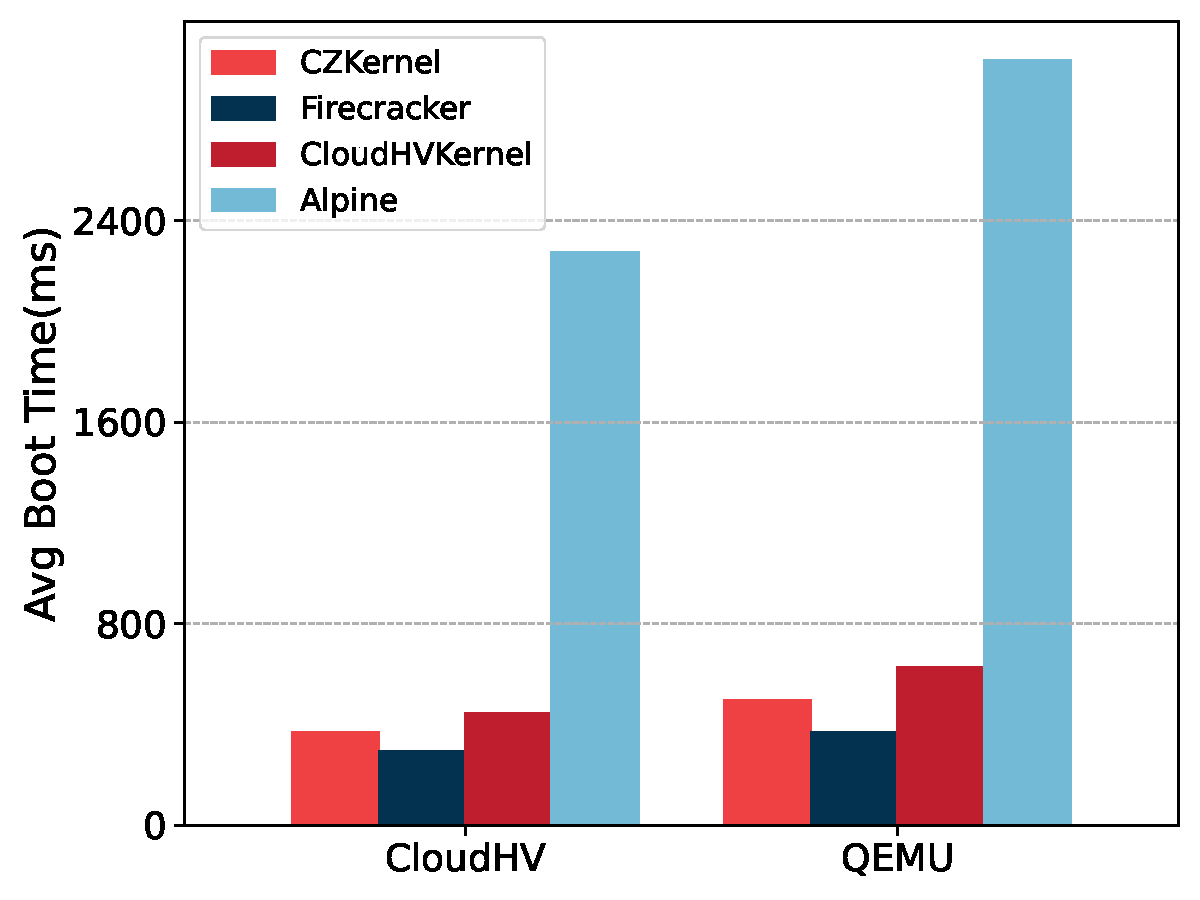
\includegraphics[width=0.5\textwidth]{avg_boot_time}
    \bicaption{\quad 不同内核与沙箱下的平均启动时间比较}{\quad Comparison of average startup times under different kernels and sandboxes}
    \label{fig:avg_boot_time}
\end{figure}

实验结果如图~\ref{fig:avg_boot_time}所示,Control Zone内核的平均启动开销相较于Alpine Virt内核最高降低了88.8\%。对比不同的虚拟机监视器的数据发现,优化效果的绝大部分来自于对内核的裁切。Control Zone内核仅支持运行容器、BPF子系统与Sched Ext调度类的最小功能,因此在启动时省去了大量非必要的工作,从而能够做到足够快速。同时,即便对于相同的Alpine Virt内核,使用CloudHypervisor相较于Qemu降低28.9\%的启动时间。观察两者的启动日志能够发现,虚拟机启动时间的差异主要来自于模拟设备的初始化上。CloudHypervisor仅针对云场景,因此相较于Qemu去除了大量的无关设备模拟。更少的模拟设备一方面减少了虚拟机监视器的启动时间,另一方面Guest内核在设备探测与初始化上花费的时间也更少。尤其在PCI子系统的初始化上,相较于Qemu,CloudHypervisor在PCI初始化上的平均时间减少了83.2\%。

\begin{figure}[!htbp]
    \centering
    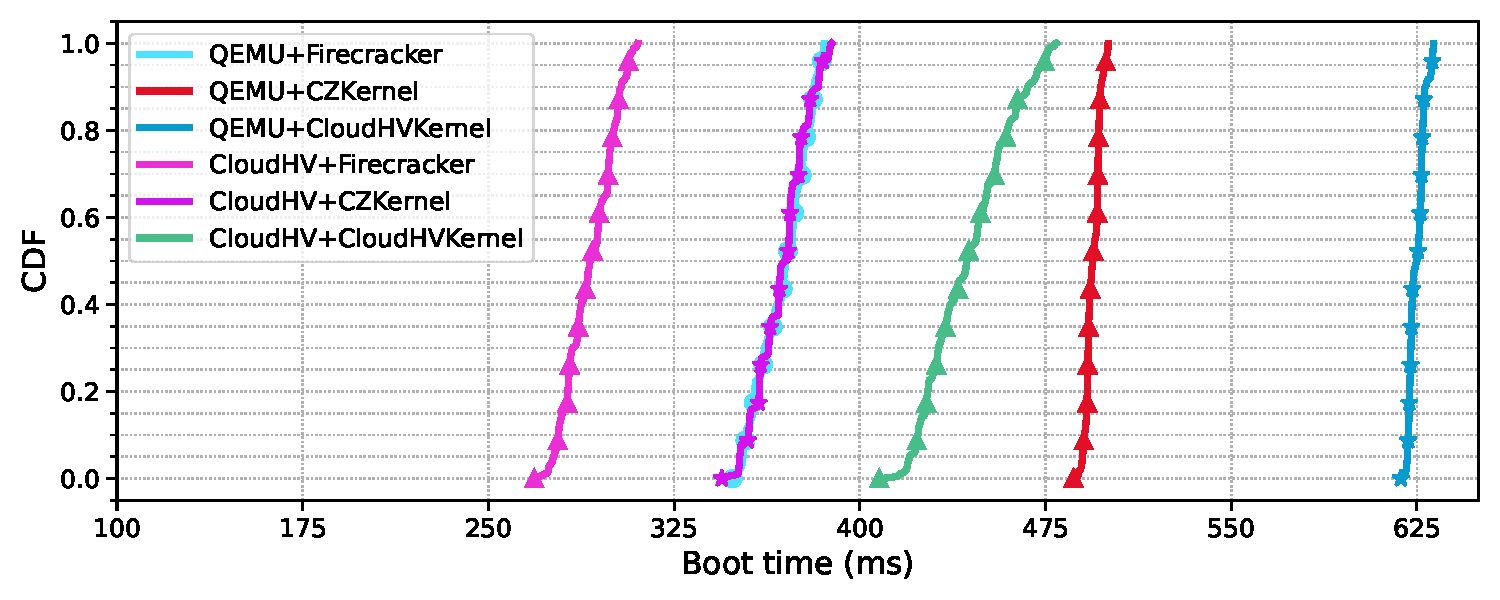
\includegraphics[width=0.8\textwidth]{boot_time_cdf}
    \bicaption{\quad 轻量化虚拟机的启动时间比较}{\quad Comparison of startup times for lightweight virtual machines} 
    \label{fig:boot_time_cdf}
\end{figure}

而对于精简内核,由于支持的PCI设备更少,因此在模拟设备初始化时间上的优化效果就并不明显。但与其余精简内核相比,Control Zone内核也存在一定优势。如图~\ref{fig:boot_time_cdf}所示,使用Qemu时,Control Zone内核相较于CloudHypervisor默认内核在启动时间上减少了20.6\%。对比两者配置差异发现,CloudHypervisor所提供的精简内核虽然去掉了大部的驱动支持,但仍然保留了如虚拟化子系统在内的配置,因此存在额外的开销。Control Zone内核由于只需要支持容器运行环境,因此能够取得更快的启动速度。但是相较于Firecracker默认内核,Control Zone即便在CloudHypervisor下也仅能达到Firecracker在Qemu下的启动时间。比较两者的配置能够发现,Firecracker内核在功能裁切上更加激进,不支持容器运行环境与BPF子系统。然而在Control Zone内核中,这些功能则是必要的。在具体使用场景中,Firecracker注重安全容器的需求,虚拟机的生命周期与运行在其中的应用绑定。但在Control Zone的设计中,Control Zone并不完全与混部应用绑定,而是一种可复用的运行环境。Control Zone在混部应用部署时启动,而在应用结束后仍然会保留一段时间,并提供给需要类似隔离环境的其他混部应用使用。因此在启动时间上花费更多的时间在Control Zone的设计中是可接受的。

\subsection{Control Zone性能开销}

实验中选择典型应用分析中的6种应用进行性能测试,分析Control Zone上实际应用的性能。在内核性能上,选择与CloudHypervisor默认Linux内核进行比较,并同时运行在Control Zone沙箱上。而在沙箱性能上,选择与在Host上以容器的形式部署的应用进行比较。

性能开销实验结果如图~\ref{fig:perf_app}所示,总体来看,Control Zone在内核性能上优于CloudHypervisor默认的Linux内核,而在沙箱性能上,Control Zone在一些应用上能够实现优于直接在Host上部署的性能。

\begin{figure}[H]
    \centering
    \begin{subfigure}[b]{0.32\textwidth}
        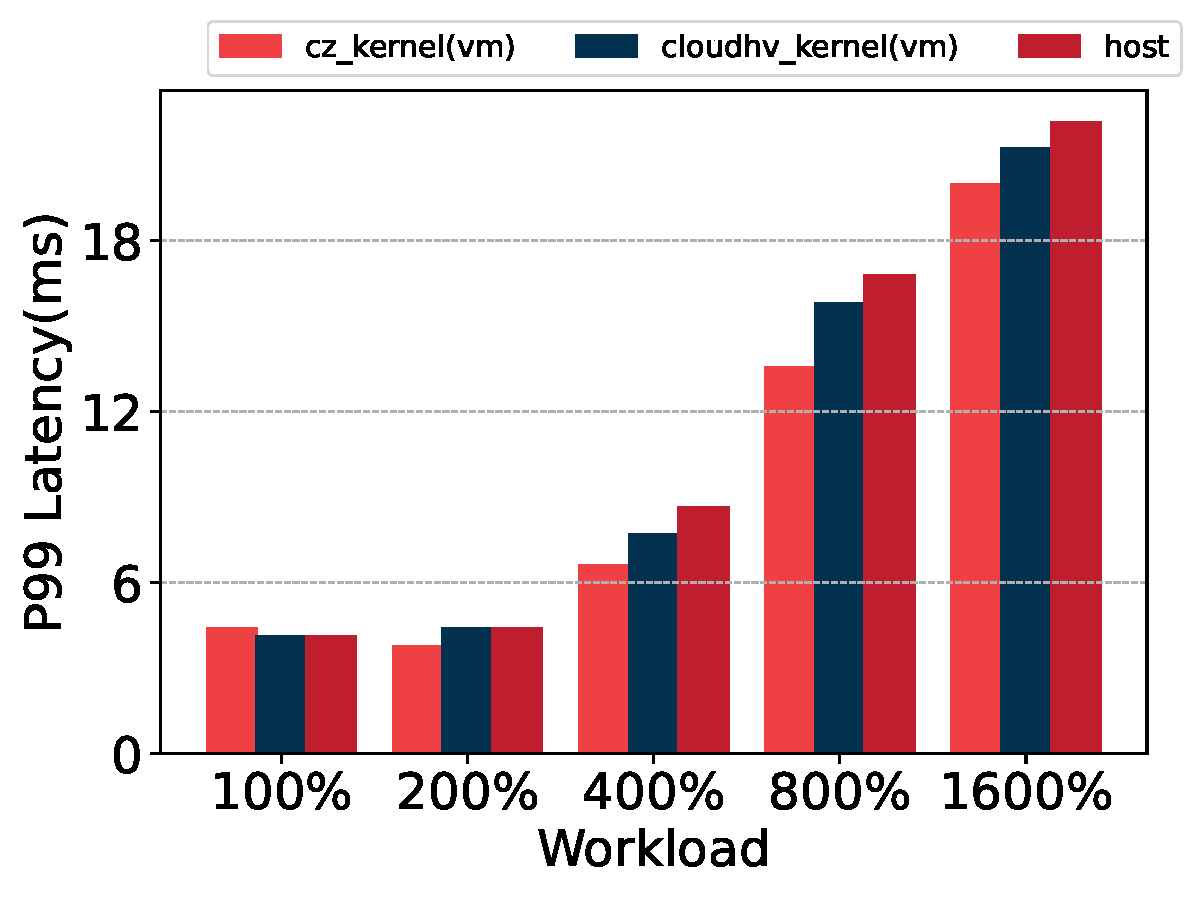
\includegraphics[width=\textwidth]{perf_redis}
        \caption{\quad Redis请求延迟}
        \label{fig:perf_redis}
    \end{subfigure}
    \begin{subfigure}[b]{0.32\textwidth}
        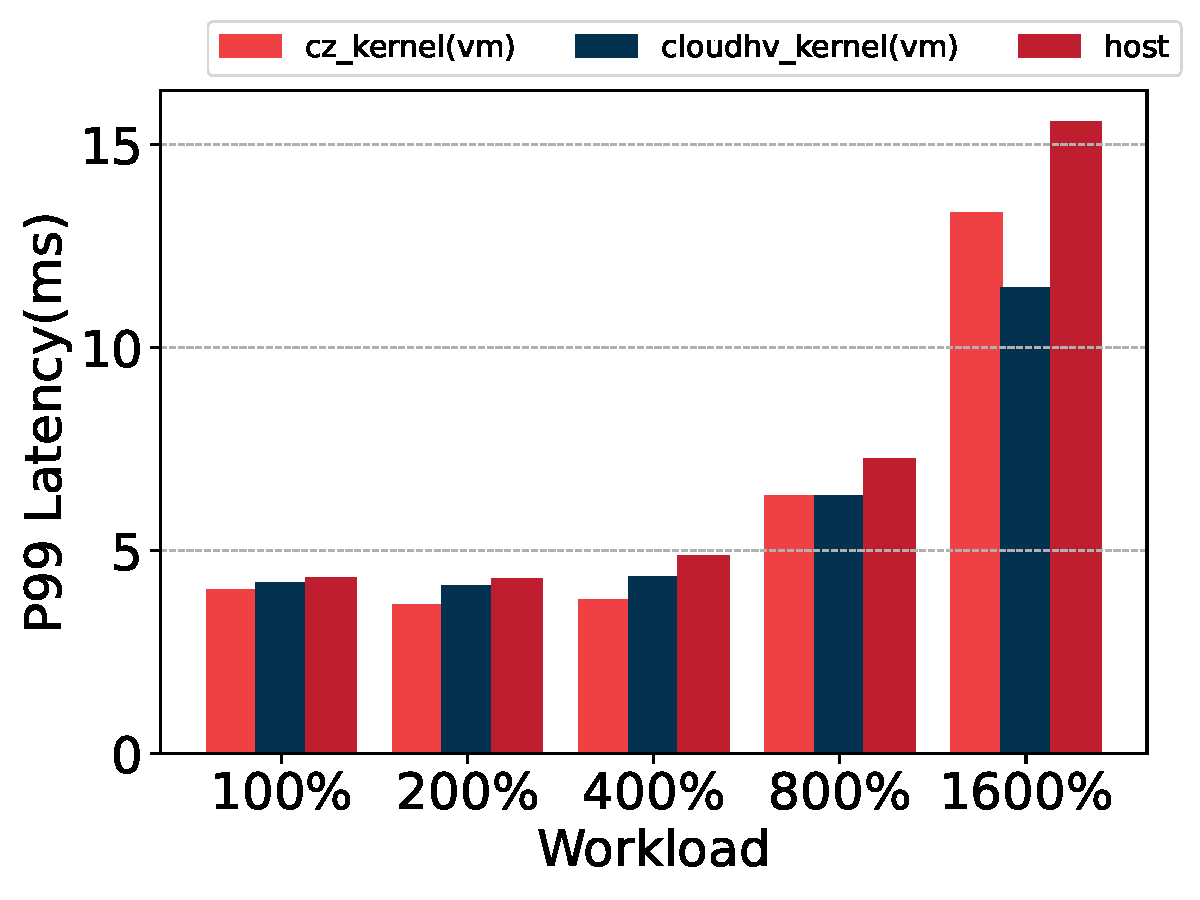
\includegraphics[width=\textwidth]{perf_memcached}
        \caption{\quad Memcached请求延迟}
        \label{fig:perf_memcached}
    \end{subfigure}
    \begin{subfigure}[b]{0.32\textwidth}
        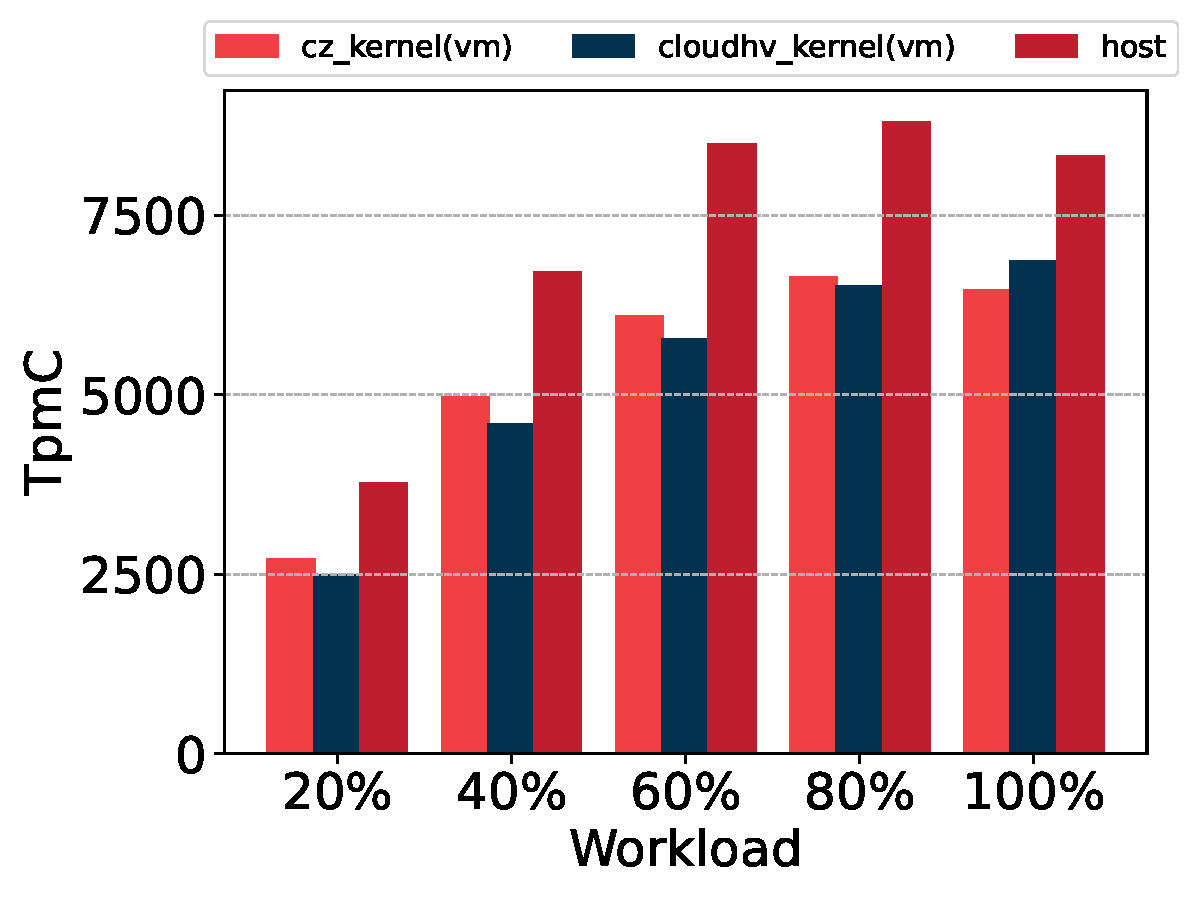
\includegraphics[width=\textwidth]{perf_mysql}
        \caption{\quad MySQL每秒事务数量}
        \label{fig:perf_mysql}
    \end{subfigure}
    \begin{subfigure}[b]{0.32\textwidth}
        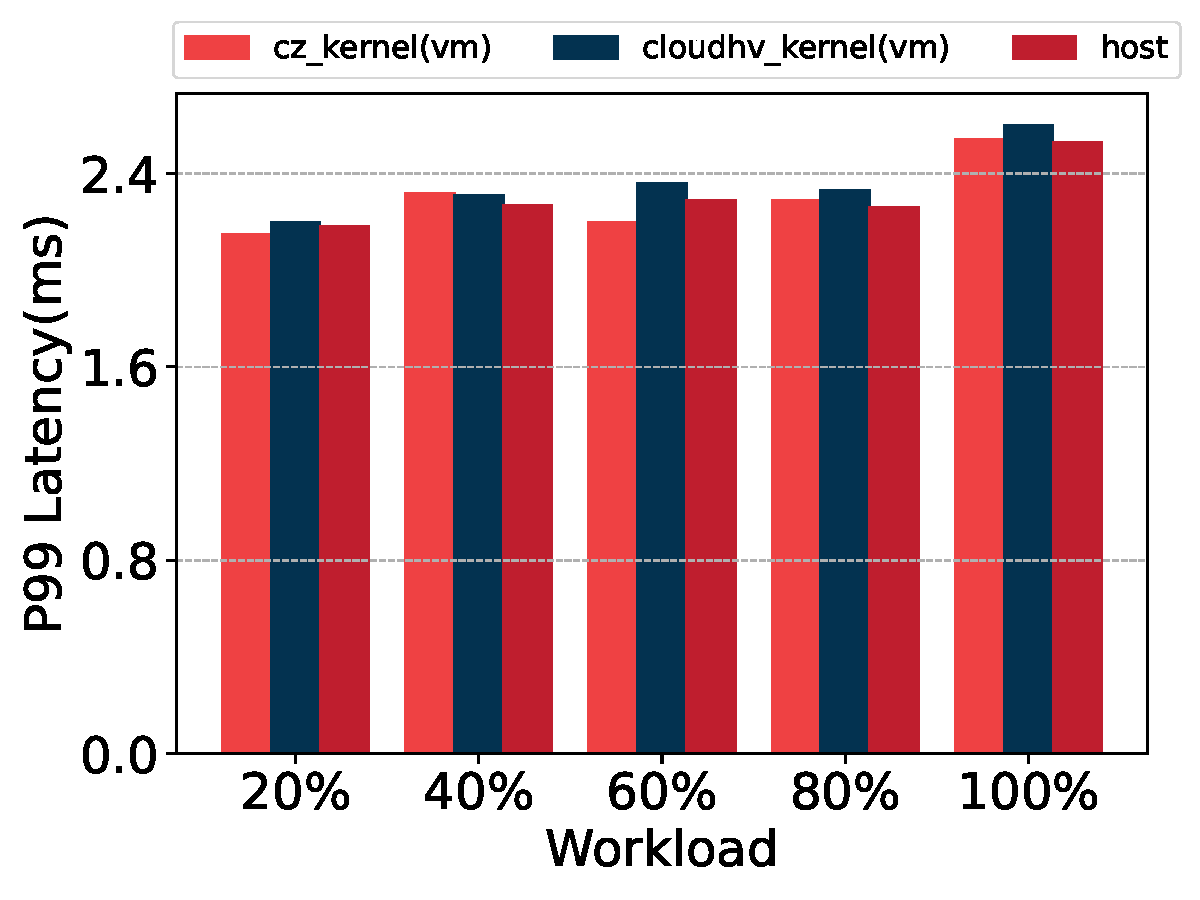
\includegraphics[width=\textwidth]{perf_nginx}
        \caption{\quad Nginx请求延迟}
        \label{fig:perf_nginx}
    \end{subfigure}
    \begin{subfigure}[b]{0.32\textwidth}
        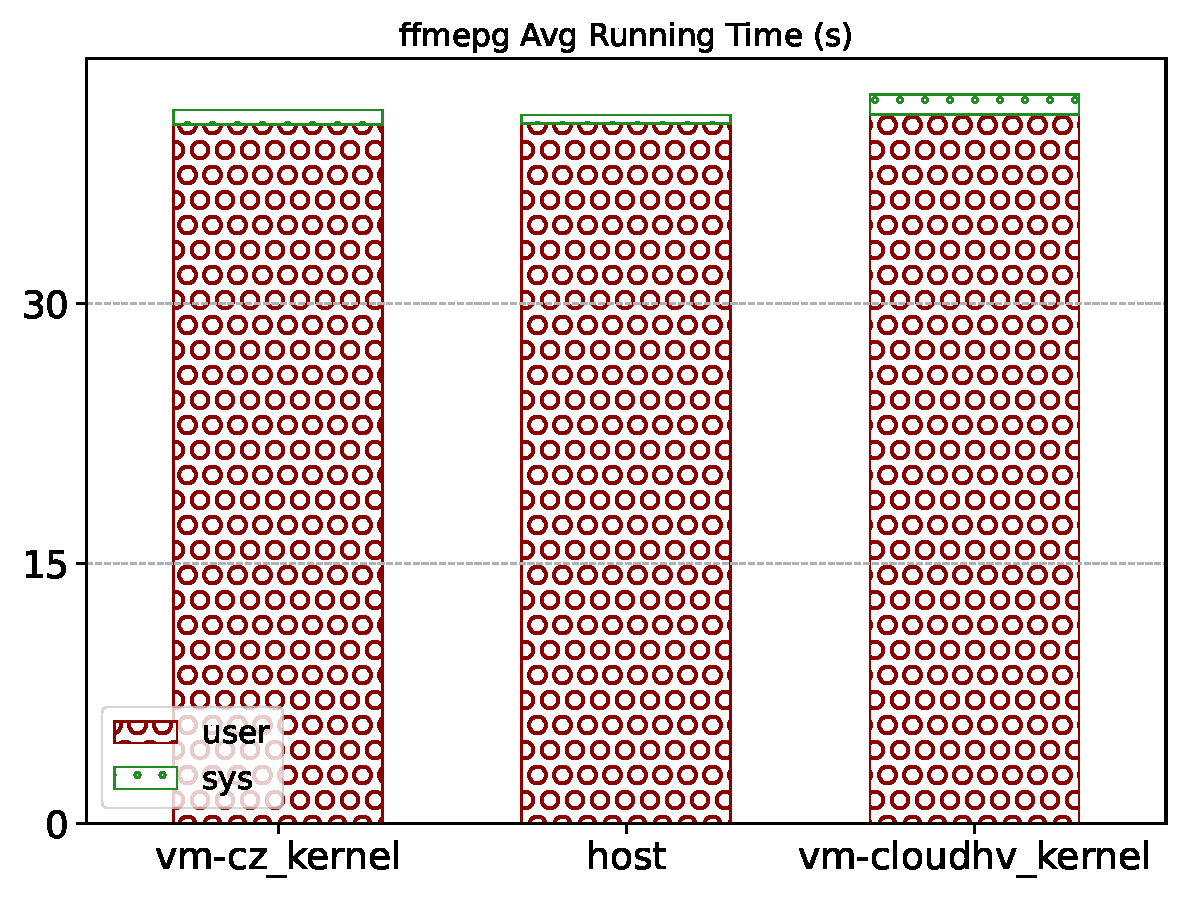
\includegraphics[width=\textwidth]{perf_ffmpeg}
        \caption{\quad FFmpeg 每秒处理帧数量}
        \label{fig:perf_ffmpeg}
    \end{subfigure}
    \begin{subfigure}[b]{0.32\textwidth}
        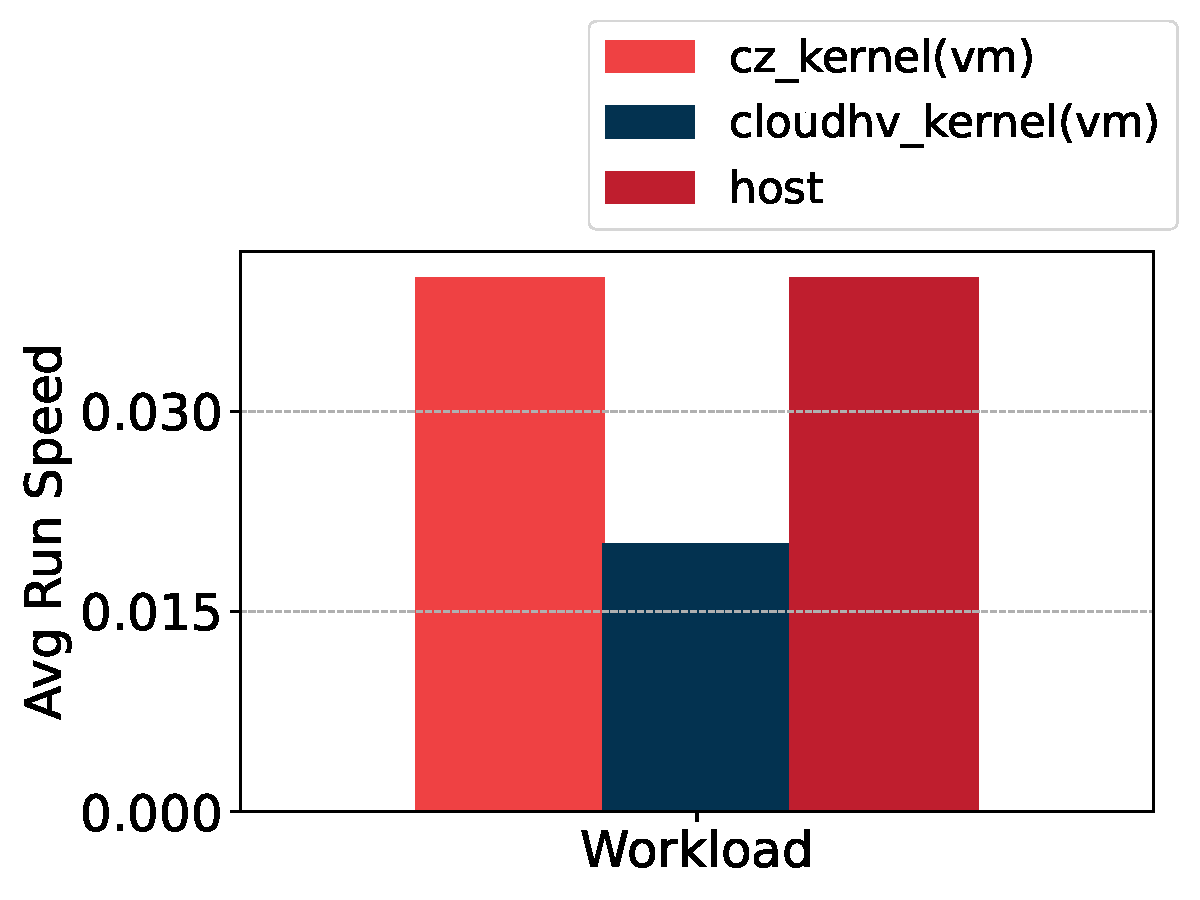
\includegraphics[width=\textwidth]{perf_graph500}
        \caption{\quad Graph500 每分钟执行数量}
        \label{fig:perf_graph500}
    \end{subfigure}
\bicaption{\quad Control Zone沙箱对不同应用性能的影响}{\quad The impact of the Control Zone on the performance of different applications}
\label{fig:perf_app}
\end{figure}

Control Zone内核仅以提供隔离的内核环境为目标,在此目标上进行的内核配置裁切能够更加激进。相较于CloudHypervisor默认内核,Control Zone内核在同样仅支持Virtio设备的同时,裁切了如Netfilter等在沙箱中不必的内核功能,从而进一步减少内核中如网络处理等关键路径的长度。因此网络应用延迟上,与同样运行在虚拟机中的CloudHypervisor内核相比,Control Zone实现了99分位尾延迟降低最高15.7\%的效果。同时,与直接运行在Host上相比,Control Zone即便引入了虚拟化开销,也能够实现99分尾延迟降低最高38.5\%的效果。

但对于一些逻辑复杂的应用,如MySQL,Control Zone存在一定的性能瓶颈。造成这一问题的核心原因是虚拟设备的性能限制。而在当前虚拟化技术中,通过SRIOV等硬件直通手段可有效地处理这一问题,因此Control Zone内核中保留了PCI总线配置以便驱动直通的硬件。

\subsection{Control Zone混部场景QoS保障效果}

性能保障实验在4 CPU、1024MB内存的Control Zone中展开,选择Qemu组合CloudHypervisor默认内核作为运行环境的对比。Control Zone中的混部方案为Memcached、stress\_ng CPU干扰应用与Control Tower调度策略,Qemu的混部方案为Memcached、stress\_ng CPU干扰。实验方式为分别在两个混部方案中运行一段时间相同的Memacached负载,并从Black Box观测系统中截取对应时间段的指标数据。

时序数据如图~\ref{fig:cpu_series_memcached}所示,包含虚拟机总体的CPU使用率、混部应用各自的CPU使用率以及Memcached的99分位尾延迟,其中红色虚线部分表示stress\_ng CPU负载启动的时间点。在干扰负载启动之前的时段,Memcached在Control Zone中的性能表现无明显差异。而在干扰负载启动之后的时段,Memcached在Control Zone中运行时的延迟需求得到了有效的保障,并实现99分尾延迟降低最高63.8\%的效果。

\begin{figure}[H]
    \centering
    \begin{subfigure}[b]{0.49\textwidth}
        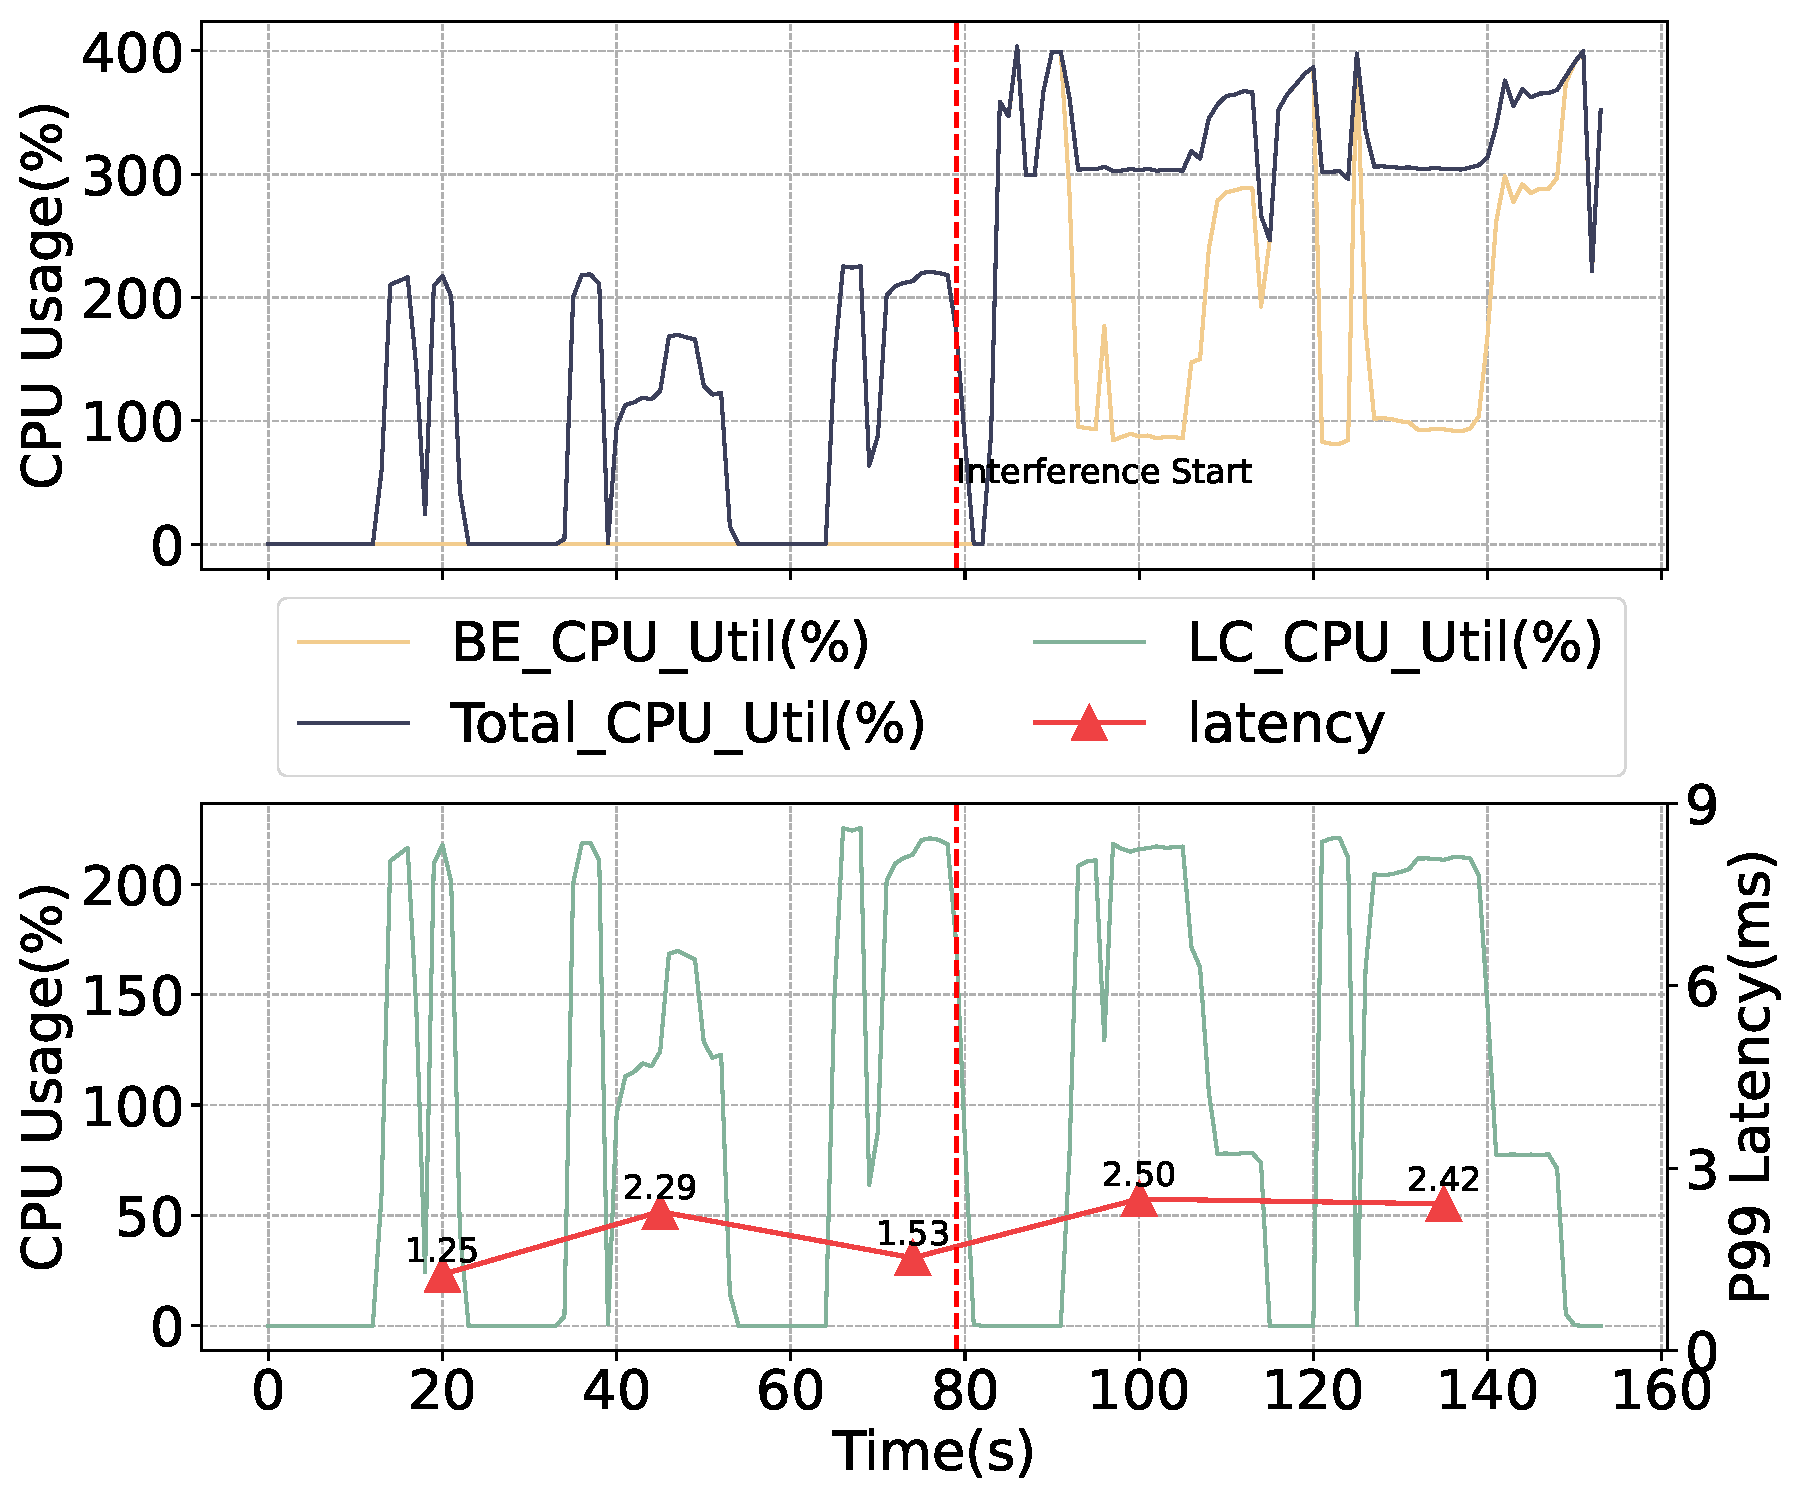
\includegraphics[width=\textwidth]{cpu_series_memcached_ct}
        \caption{\quad Control Zone混部性能}
        \label{fig:cpu_series_memcached_ct}
    \end{subfigure}
    \begin{subfigure}[b]{0.49\textwidth}
        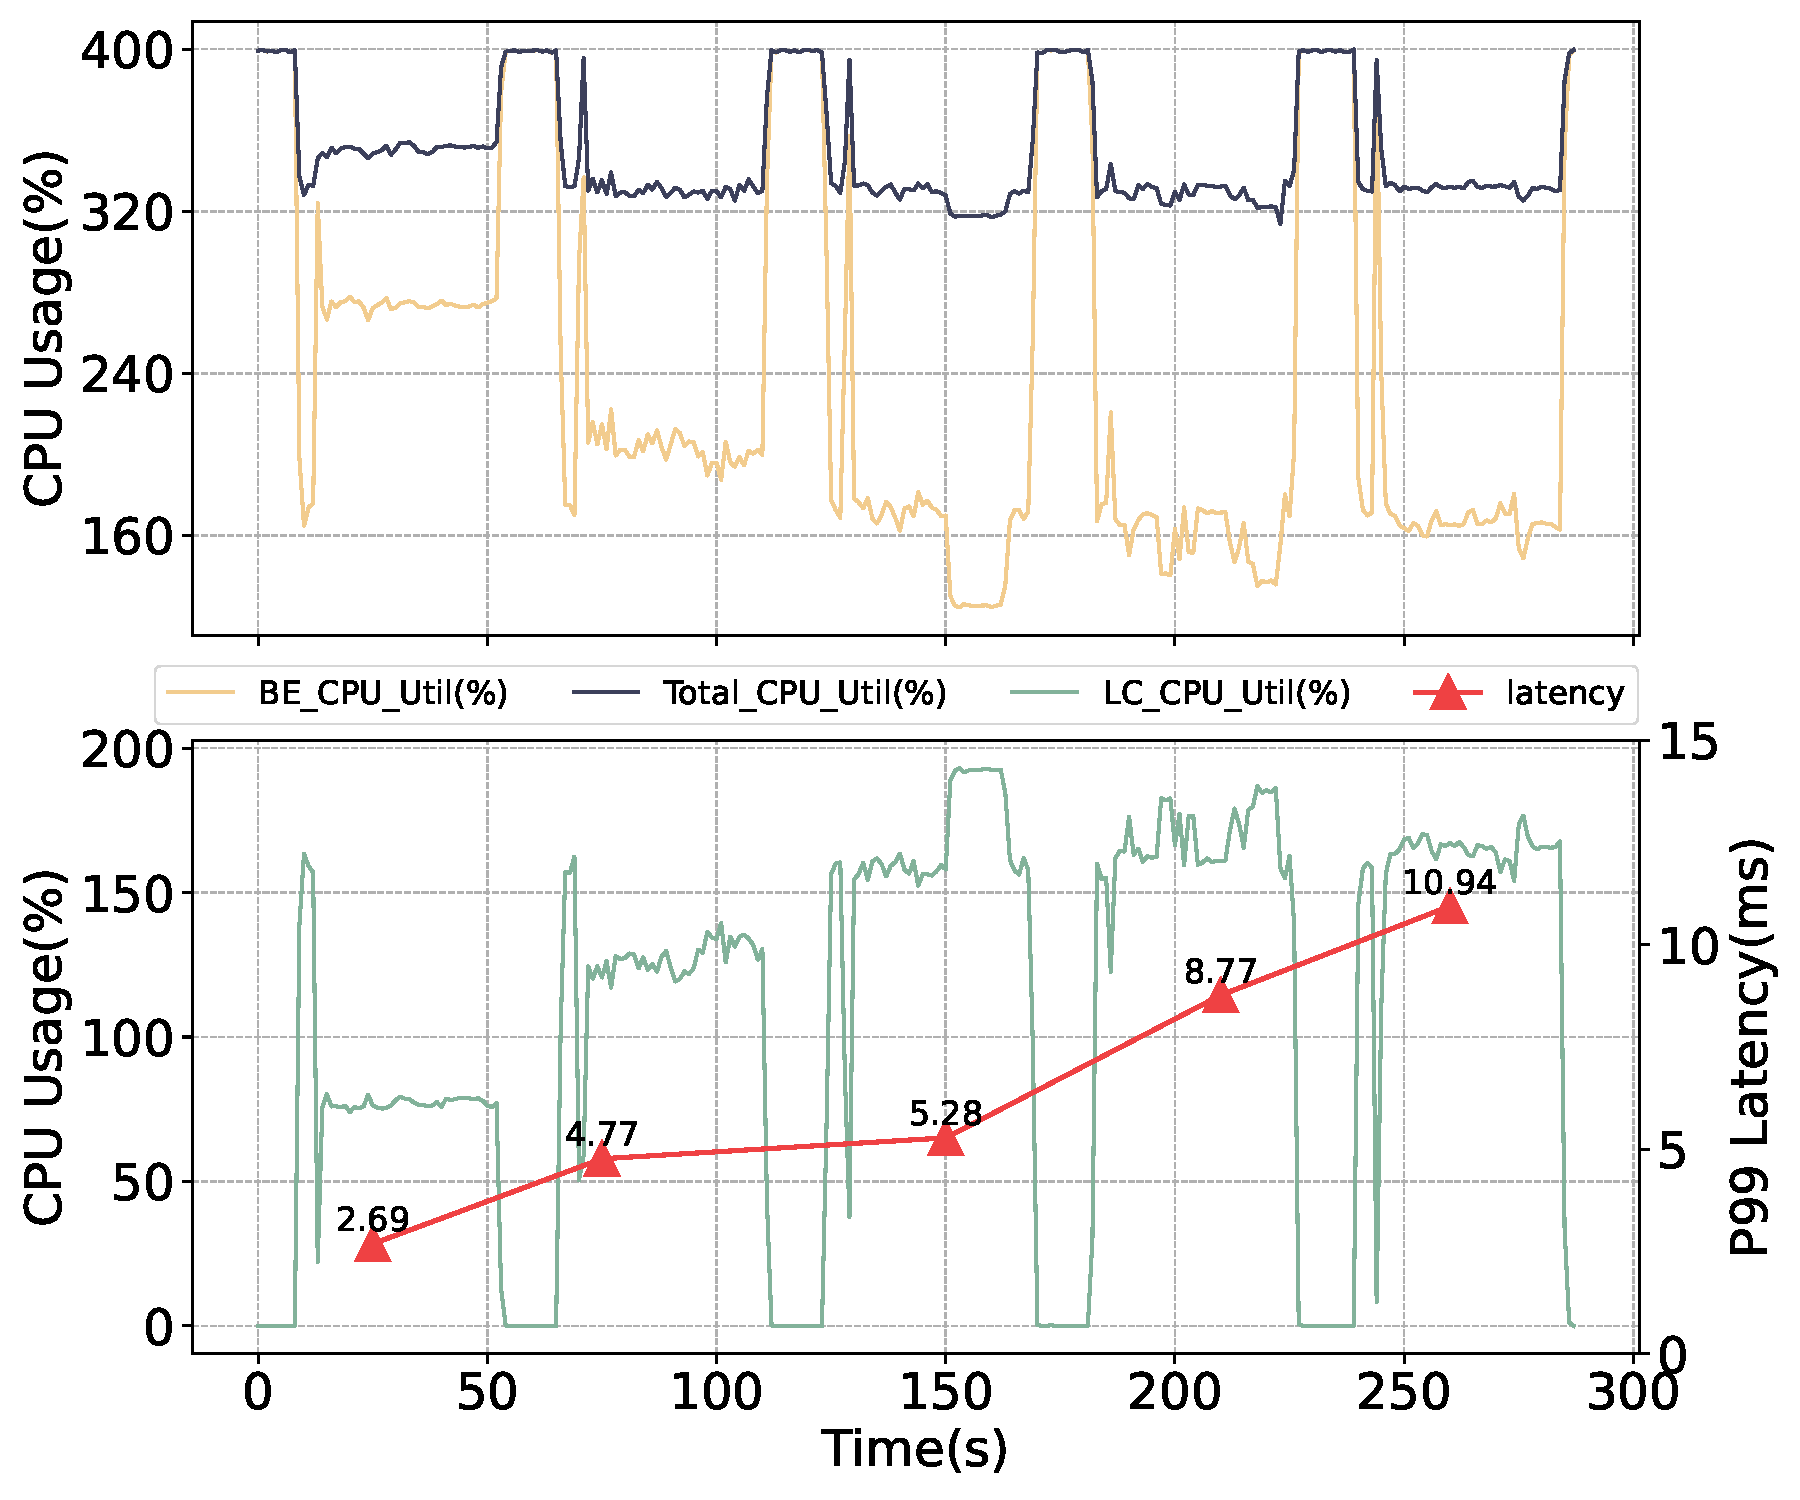
\includegraphics[width=\textwidth]{cpu_series_memcached_eevdf}
        \caption{\quad Qemu + CloudHV Kernel混部性能}
        \label{fig:cpu_series_memcached_eevdf}
    \end{subfigure}
    \bicaption{\quad 混部场景下Control Zone对Memcached服务性能的保障效果}{\quad Effectiveness of Control Zone for Memcached QoS guarantee in co-location}
    \label{fig:cpu_series_memcached}
\end{figure}

而从CPU资源分配的角度上来看,Memcached在Control Zone中运行时能被更优先地分配CPU资源,从而能够更好地进行请求处理,实现延迟的降低。与此同时,虚拟机总体CPU使用率却没有明显下降,这得益于Control Tower调度策略对于高优先应用CPU资源使用的感知,并通过合理的CPU分配实现高优先应用的性能保障。

% 补充实验
% - 总体性能指标
% - 混部场景变化实验
% - 同时运行实验

\section{本章小结}

本章首先介绍了运行时调度可变的沙箱Control Zone的基本概念,以及其对数据中心中单节点混部场景的处理方式,即结合外侧虚拟机资源隔离与内部Control Tower任务调度策略。

随后介绍了Control Zone轻量级虚拟机的实现,以及在实现中为解决引入虚拟化带来的开销做进行的工作,包括对虚拟机监视器的轻量化以及对操作系统的精简。

然后介绍了沙箱中的czctrl、czmanager、czdaemon等组件及其主要功能,并详细阐述了Contorl Zone的隔离能力以及Control Zone生命周期管理中各个组件的协作过程。

实验设计中,在沙箱启动开销上,比较了Control Zone虚拟机的启动时间,通过在Hypervisor、Guest OS上的裁剪优化,Control Zone能够达到与领先轻量级虚拟化相近的水平。而在性能开销上,选择6种应用进行性能测试,Control Zone沙箱在多数应用上都取得了更好的性能,同时依托内核上的裁切,能够弥补虚拟化所带来的开销,并达到应用性能优于在Host上直接部署的效果。

而在混部性能保障上,Control Zone部署混部应用能够利用Contorl Tower调度策略的灵活性与调控能力,通过更符合混部场景的CPU资源分配策略,能够实现高优先应用99分尾延迟降低最高63.8\%的效果。